%
% This is a borrowed LaTeX template file for lecture notes for CS267,
% Applications of Parallel Computing, UCBerkeley EECS Department.
% Now being used for CMU's 10725 Fall 2012 Optimization course
% taught by Geoff Gordon and Ryan Tibshirani.  When preparing 
% LaTeX notes for this class, please use this template.
%
% To familiarize yourself with this template, the body contains
% some examples of its use.  Look them over.  Then you can
% run LaTeX on this file.  After you have LaTeXed this file then
% you can look over the result either by printing it out with
% dvips or using xdvi. "pdflatex template.tex" should also work.
%

\documentclass[twoside]{article}
\usepackage{graphicx}
\usepackage{listings}
\lstset{language=C}
\title{Computer Systems}
\date{}
\author{}
\begin{document}
\maketitle
\section{Introduction}
\subsection{Networks}
The internet is essentially a network of networks. Communication infrastructure enables distributed applications. Project 2 will likely be a multi-threaded server. A protocol is used to establish connection first, and then the data is transferred from the client to the server. We need to use the port number and the I.P. address of the server for communication.
\subsection{Operating Systems}
The OS provides a much higher level interface. The OS plays referee, preventing people from stepping on each other. The CPU scheduler provides the illusion that multiple programs can run on one CPU at the same time. Virtual memory provides an address that is larger than the size of the physical memory. It also provides a file system, so the programmer doesn't have to think about the sectors on the disk.
\subsubsection{Process Management}
\textbf{Exam Questions:} Define processes and multi-programming; managing processes in Unix/Linux; the user-kernel distinction; system calls in Unix/Linux; threads\\ \\
A process is a program execution; a program is static, a process is dynamic. For example, like cooking, the recipe itself is static and is like a program but the act of cooking itself is dynamic and therefore is like a process. Processes have three segments: the stack, the data and the text (the actual code). The stack is where the variables are and the the heap is where all the mallocs are.  Ctrl-Z doesn't kill the process, it just puts it to sleep (it keeps running in the background). Every process that runs has a parent as it had to come from somewhere.\\
If several processes are to be active at the same time, there has to something that has to keep them in check; enter the \textbf{kernel}. Note: the kernel is \textbf{not} itself a process.\\
CPUs have two modes: the user mode and the kernel mode. The program status word (PSW) gives the current mode. The code running in user mode cannot issue privileged instructions but code running in kernel mode can. The user-kernel distinction is the core of the security in a given OS. To go into the kernel mode from the user, like if we have to print something in C, the trap bit is initiated and then the code enters the kernel mode, and the code then runs in kernel mode. System calls are used to allow users to ask for the kernel to execute privileged instructions or access privileged memory locations. Examples are \texttt{open, read, write, close, fork, exec, exit, wait} etc. \textbf{Need to know these commands.} There are systems calls for everything from process control to file management, device management, communication etc. \texttt{printf} in C is not a system call, it call \texttt{write()}, therefore providing that extra level of abstraction. For example, if we call \texttt{read()} the program gives the control to the kernel, which does everything and then the controls returns to the program. \\ \\
\texttt{fork()} creates a new process with the exact copy of the parent. If \texttt{fork()} returns 0, then the child process was created. Exec* is also a systems call and is used to run other programs, it replaces the address space of the process. Also note that this entire program is non-deterministic, as in we don't know which is going to print out first, the parent or the child. This is because they both are separate processes and the processor may decide to put one ahead of the other depending on the circumstances.
\subsubsection{Interrupts}
When a hardware device needs the attention of the CPU e.g. if it has finished doing its task, it makes an interrupt. When an interrupt occurs, the CPU's hardware takes the values in the program counter and the program status word registers, and saves them in privileged parts of the memory reserved just for this purpose. The interrupt handler must do several tasks: 
\begin{itemize}
\item save the rest of the status of the current process
\item service the interrupt
\item restore what it saved
\item execute a \emph{return for interrupt} or similar instructions to restore whatever the hardware saved when the interrupt occurred
\end{itemize}
The \emph{interrupt vector} is an area of memory that stores the program counter, the PSW and on some machines the stack pointer for use when the interrupt occurs, this address is wired into the CPU.

\section{Process Management}
\textbf{Exam questions:} \begin{itemize}
\item Difference between user and kernel mode?
\item Why have the distinction?
\item What are the security mechanisms?
\item What are the three main purposes of an OS? Provide an environment for the users to run their programs on hardware in an efficient manner; to allocate separate resources of the computer as needed, the allocation process should be as efficient as possible; as a control program it serves the purpose of supervision of the user programs to see if they are running properly without any errors and management of the operation and control of the system I/O
\item What is the purpose of a system call? They allow user-level processes to request services of the OS.
\item In Linux, what system calls have to be executed by a command interpreter or shell in order to start a new process? A \texttt{fork()} system call is followed by an \texttt{exec()} call needs to be performed to start a new process. The \texttt{fork()} call clones the currently executing process, while \texttt{exec()} call overlays a new process based on a different executable over the calling process.
\end{itemize}
Remember a program has a program code, global data, heap and stack. What is going on when we use a signal? The basic cycle of execution is Start; fetch next instruction; execute instruction; loop back to fetch next instructions until there are no more left and then finally finish the program. To extend further: whenever an instruction is executed, there is a check to see if there was an interrupt issued. \\ \\
Any given interrupt has a different Interrupt Priority Level (IPL), and the CPU only services the interrupts that have a higher IPL than the process currently running. The OS executes the interrupt at the IPL of the interrupt handled. Usually we put the clock at the top followed by networks, tapes and then disks. \textbf{True interrupts} come from hardware outside the CPU and \textbf{Pseudo-interrupts} come from inside the CPU, like a divide-by-zero error. Each type of pseudo-interrupt has its own entry in the interrupt vector. For hardware syscall instructions, examples are TRAP, and INT 2E. A system call instruction causes a \textbf{synchronous} except (or \emph{traps}), other examples are divide-by-zero, bus error, page fault etc. Interrupts are \textbf{asynchronous} exceptions, examples are timer, disk, ready, network etc. On a system call, exception or interrupt the hardware/OS enters kernel mode with \emph{interrupts disabled}; saves PC, then jumps to the appropriate exception handler in the kernel. A systems call runs in kernel mode, but it \emph{checks for permissions first}.
\subsection{Threads}
\textbf{Definition:} a sequential execution stream within the process (sometimes called a "lightweight process"). Threads are the basic unit of CPU utilization - including program counter, register set and stack space.\\ \\
Some OS's provide functionality for sharing by dividing the notion of a process into two components: a thread and a container for the thread. Thus, a process has one container, but may have more than one thread, and each thread can perform computation (almost) independently of the other threads in the process. \emph{Note: only one thread can run at a time.} An example is a word process or a multi-threaded server which creates a new thread to deal with each of the requests it gets. For any given program, information such as the code, data and the files are shared but each thread has its own stack and register. The data shared by threads is address space and memory - code and data section; contents of memory (global variables, heap); open files; child processes; signal and signal handlers. Threads have their own copy of: program counter, registers, stack (local variables, function call stack), state (running/waiting). Threads can easily communicate with each other, and there is less overhead when compared with making multiple processes. Look at the \texttt{pthread} library for creating threads in C. Global variables are shared across threads. \emph{Thread switches can occur at any point.} Thus, another thread could modify shared data at any time; therefore there is a need to \emph{synchronize} threads to avoid such problems.
\subsection{Process Scheduling}
\textbf{Exam questions:}
\begin{itemize}
\item Process states (and the use of PCB)
\item Context switching
\item The use of scheduling algorithms
\item Explain the performance characteristics of particular algorithms
\end{itemize}
A process can be in one of three states: \textbf{running:} actually using the CPU, \textbf{ready:} runnable; temporarily stopped to let another process tun and \textbf{blocked} unable to run until some external event happens. Note that a process \textbf{cannot} go from being ready to blocked. Saved states of processes are stored in the kernel in the \emph{process table} which has a slot for every process. Some entries are:
\begin{itemize}
\item process id
\item process state
\item user id and other privilege information
\item start addresses and sizes of memory areas
\item CPU time used and other accounting information
\item priority
\item working directory
\item list of open files and information about them
\item space for saved copies of registers (including PC, PSW and SP)
\end{itemize}
To create a process first memory is allocated for it; the process control block is initialized; the process is inserted into the Ready queue; sometimes running time is estimated; its memory requirements are sometimes analyzed and finally, the its first part is loaded into memory. \\ \\
When an interrupt occurs and a running thread is set to ready, and the CPU comes back after the interrupt the highest priority thread is restored, sometimes this is not the thread that was running before, if this is the case, then this event is called a \emph{context switch} and the previously running thread was preempted. \emph{Processes and threads are not aware of interrupts or context switches.} \\ \\
For any scheduling lgorithm it must be fair: every process/thread should get its fair share of the CPU; throughput: should maximize the number of jobs processed per time; response time: should minimize waiting for interactive users; turnaround time: should minimize waiting for batch jobs.\\ \\
FCFS works well when job times are similar but it is unfair to short jobs. Shortest first has a good turnaround time but it may starve long jobs. R.R. keeps a list of ready threads and allocates a quantum of time to each of them. If a thread is still running at the end of its quantum, it is put back in the queue. If we have a short quantum we have good response time, poor throughput, good for interactive systems; if we have long quantum we have poor response time, good throughput, thus great for batch systems.\\ \\
A S.R.R. works like R.R. except it doesn't put jobs in the ready queue until demand for the CPU is "acceptably low". Thus, S.R.R. can approximate either F.C.F.S. or R.R.\\ \\
There is also priority scheduling which assumes that each thread has a priority and it always runs the thread with the highest priority. Note that the process's absolute priority doesn't matter as much as its priority as relative to the processes its being compared with.

\section{Memory Management}
\textbf{Exam Questions:}
\begin{itemize}
\item Fragmentation
\item The mapping between physical and virtual memory
\item Paging: page faults, page tables, page replacement algorithms
\item Working set
\end{itemize}
The main functions of a memory manager are: to keep track of allocated and free 
parts of memory, to allocate memory, to protect memory from unwanted access and 
to simulate bigger main memory by automatically moving data between the disk and
 memory. There are different types of memory from smaller \& faster to larger 
 \& slower: register, L1 cache, L2 cache, main memory, local secondary storage 
 and remote secondary storage. The parts of the disk used to store process 
 information on the disk are called the \emph{swap space} as total size of all 
 processes may exceed total memory size. As processes are added and removed from
 memory, if there is a smaller process in memory than the previous one, the too-small 
 space becomes unusable and over time a lot of these \emph{holes} start to 
 appear, this problem is called \emph{external fragmentation.} One way to solve 
 this is to move all the processes into one contiguous area in memory, this is 
 called \emph{memory compaction.} This is not done as memory speed is very low 
 as compared with the CPU speed. The program is unaware of the fact that the 
 address it has and the physical address of a memory location are different 
 as the OS adds a base register (an offset) to the addresses generated by the 
 program. Base and limit registers guarantee security if the addresses generated 
 by a program are always checked with the limit register and an exception raised 
 if outside limit; and the base and limit registers are only modifiable in kernel 
 mode.\\ \\

A program assumes that all its code and data are in main memory when running 
and the code and data are stored in contiguous locations. These assumption also 
cause external fragmentation. Virtual memory is applied via \textbf{paging} or 
\textbf{segmentation.} Paging relies on the difference between physical and 
virtual/logical addresses and uses a \emph{memory management unit} (MMU) to do 
the translation. CPU's typically provide a way to access physical addresses 
directly without MMU in kernel mode. MMU is usually in the CPU or close to it. 
The virtual address space is the set of addresses a program on a machine may 
generate. \emph{Each process has its own virtual address space.}\\ \\

A paged system divides both physical and virtual addresses into pages. It maps 
a virtual page to a physical page, also called a \textbf{page frame.} When a 
virtual is moved multiple times, it may be loaded into different page frames. 
Since the memory allocated to a process is an integral multiple of page size, 
there is almost always going to be some space wasted, this is called 
\textbf{internal fragmentation.} In a paged systems an address is 
\emph{pageNumber * pageSize + offset}. The page size in bytes is: 2 raised to 
the power of (BitsInTheOffset). The information required to do the mapping is 
recorded in a page table and \emph{each process has its own page table.}\\ \\

Usually a page table entry has:
\begin{itemize}
\item a physical page number
\item a valid bit to check whether the virtual page is in memory
\item a referenced bit, whether the page was referenced before
\item a modified bit
\item read, write and execute permission bits
\end{itemize}
The physical page will only be constructed by the MMU if valid bit is true and the permissions permit memory access. It will then set the referenced bit and also the modified bit if it was a write. If either conditions isn't met is raises a \emph{page fault} exception, to be handled by the kernel.

\section{Memory Management}
\textbf{bits in offset = size of page}\\ \\
If the valid bit is zero and the OS must:
\begin{itemize}
\item suspend the process
\item free up a page frame if required
\item load the virtual page
\item cause MMU to map that virtual page
\item restart the process at the \emph{same} instruction
\end{itemize}
Now we need two memory accesses: the PTE and to access the data. To optimize we use \textbf{translation lookaside buffer (TLB)} which serves as a cache holding copies of recently accessed PTE's. To avoid overlapping of TLB entries it is cleared at every context switch so that there is no conflict like process 1 and 2 having same virtual addresses pointing to different physical addresses.\\ \\
A scheme used was splitting the page into two, for code, heap at the start and the stack at the end, but this can't handle dynamic linking and shared memory operations. Thus, a \emph{page table directory} is always in memory when a process runs whose entries point to page table fragments which may be in memory or in disk. \\ \\
For a split system we must know the physical address of the each half of PT and their lengths. For directory, we want to know the its physical address, its length and fragment length. A \emph{page table base register} in the CPU has the first word of the currently running process. In most computers, the kernel is actually a part of the address space of every process, a virtual address with high bit set is system space and user space, otherwise. There is 1 PT for system space and 1 for each user processes.\\ \\
The page fault handler must be kept in memory. If the TLB misses the lookup shouldn't go through the MMU in a usual way. If the chosen page to be replaced has been modified (modified bit changed) then the OS must first write the changes to disk before taking it out of the memory. All page replacement algorithms assume that the near future will be the same and the near past. Two techniques are used: \textbf{spatial locality:} locations around a recently referenced location are likely to be used; \textbf{temporal locality:} if a location has been referenced lately, it will be referenced again.\\ \\
Page replacement policies: \textbf{optimal} which chooses the page whose reference is going to be the furthest in the future, and established the upper bound on how good an algorithm can be; \textbf{random} which picks a page at random; established the upper bound on how bad an algorithm will be; in some cases can't do better than this.\\ \\
The FIFO algorithm is simple but disregards locality and throws out even heavily used pages. The LRU algorithm picks the least recently used page, but it requires us to keep time stamps, which doubles memory accesses, so it isn't used. The LFU keeps a counter for each page and adjusts them at each clock interrupt but a highly used page is left in memory, even if no longer required. The clock algorithm slowly sweeps through memory clearing referenced bits, if a bit is already clear, the page is marked for replacement. A second and minute hand is used in practice for resetting and checking; they are separated by fixed page numbers or milliseconds.\\ \\
A free page pool can be used by having a list of clean, ready pages which are filled in and then the next page to be removed is found; this almost always improved performance. Paging in a dirty page requires two steps: copy to disk and write new. The page write daemon can find dirty old pages, write them to disk and put them in the pool.\\ \\
Smaller memory size lead to higher faults. If the processes in memory is too high then we get a lot of page faults and the waiting queue will be longer and CPU will be underutilized; this is called \textbf{thrashing}. If the OS knows about this, it should avoid bringing in new processes and take steps to end it.\\ \\
The principle that a process shouldn't run until the set of pages it needs regular access to are in memory is called \textbf{the working set principle.}. Also called the minimum number of pages necessary to get it to start. Whenever a program goes from one "section" to another, we will see a sharp rise in the working set size; we should accommodate for this by having the "normal" page fault rate band wide enough.\\ \\
\subsection{Process Creation}
Create processes by issuing a system call with the new process and its attributes or issue a call to clone the current process. Fork is good as it allows for environment setting before execution and can use all information from the parent to do this. Fork is bad as the cloning work done is wasted. \texttt{vfork()} borrows the address space of the parent instead of creating a new one, but child can screw with parent's address space size and contents. At \texttt{fork()} time the OS only copies the PT and sets it read-only and copy-on-write. If some tries to write to read-only page, the COW bit is checked and if set:
\begin{itemize}
\item copies the page
\item sets the write permission bits and resets the COW bits in both PTE's
\item restarts the faulting instruction
\end{itemize}

\section{File Systems}
\textbf{Exam questions:}
\begin{itemize}
\item The purpose of a file system? Application in Linux/Unix
\item File permissions
\item The use of file descriptors
\item File allocation methods including FAT and indexed (use of i-node)
\end{itemize}
The layout is (high-level to low) application programs, logical file system, file-organization module, basic file system, I/O control and devices. Collection of bytes stored on disk is called a file. Unix always views files as \emph{sequence of bytes.} Some file attributes are:
\begin{itemize}
\item Name - only info kept in human-readable form
\item unique id
\item type
\item pointer to location
\item size
\item protection - who can read, write, execute
\item time, data and user id - data for protection, security and usage
\end{itemize}
An inode contains all file info in Unix like: type, owner, group, permissions, time of last access, last modification time, last inode change, size and disk addresses. In Unix a directory is just a file maintained by the kernel. We use B-trees for speed mapping of inode and file names. A Unix filename is just a sequence of names with slashes which is converted to inode number by looking at each component. The kernel caches the pathname translations for speed.\\ \\
The same inode (file) may be referred to from more than 1 directory entry which then belongs to each of them equally, each reference is called a \textbf{link}. \texttt{ln} in Linux. Hard links can only point to regular files, not directories as each directory has its own set of inodes. Symbolic link is \texttt{ln -s} and is a special kind of file that contains a filename, whenever it's opened, the kernel sees the link kind in the inode and opens the filename instead.
\subsection{Permissions}
For \texttt{chmod} u is user; g is group and o is others. For the number 4 is for read, 2 for write and 1 for execute; from LHS of the number we have the owner, group and other. The format is \texttt{rwx}, each are set in binary. Each user is part of one or more groups; each group has a unique id and name separate from user id and name. If a user is part of more than one groups, one group is primary, the rest, secondary. User info is in \texttt{/etc/passwd} and group info is in \texttt{/etc/group}. The OS must know which subjects are authorized to perform what operations on which objects. Subjects are users or processes executing on their behalf; objects are files, areas of memory etc. There is not a full list as it would be too long so OS's keep the info with the objects or the subjects. An application is the \textbf{Access control list or ACL} which stores the info with the file itself and the ACL is searched to find the user and his/her permissions.\\ \\
A process/user can look into a directory if the 'x' is set, checks 'w' to create and delete files. When a mask is created, the unmask number is subtracted from the \texttt{chmod} number. The unmask facility is  a mechanism and default unmask is a policy. When the \texttt{setuid} bit is on the program is called a setuid program and can do commands that the user of that id can do; same for setgid. The \texttt{su} command is substitute user and \texttt{sudo} is superuser do which just runs the command line program as setuid to root.\\ \\
A file is an abstract data type with: create, write, read, reposition within file, delete, truncate, open (fi) which searches the directory structure on disk for entry fi and move the content of memory to memory and close (fi) move to the content of entry fi in memory in directory structure on disk. In Unix the input/output stream is referred to by a file descriptor: a small integer. \emph{The kernel uses the file descriptor to index into a table representing the process's open files.} It is impossible to do operations on a file with the kernel's permission. Unix system call for files are \texttt{open, read, write, close}: checks if operation permitted and then returns descriptor, read a given number of bytes into a given buffer and then return bytes read, writes n bytes to given file from buffer and make descriptor unavailable. Files are created in Unix at zero size and write beyond the current size.\\ \\
The kernel maintain a \emph{current offset}: distance from start of file to next byte to read/write. Access files randomly using \texttt{lseek} by changing the current offset. The Unix kernel keep s three main kinds of tables for files:
\begin{itemize}
\item open file table: global table containing one entry for each open without a close, and each entry with current offset
\item descriptor tables: small per-process table, maps descriptors of that process to open file table entries
\item active inode table: global table with information about every active file
\end{itemize}
The per-process file descriptor table is copied when a new process is created via \texttt{fork()}. Every program opened by the shell can count of \texttt{stdin, stdout, stderr} descriptors open.\\ \\
In Unix the drive is divided into partitions, which the kernel uses as a virtual disk. A partition may serve as a component of swap space or hold a file system; which is a tree-structured hierarchy of directories. Unix allows one file system to be mounted on top of a directory is some other file system, the root directory of the mounted file system conceptually replaces the mounted-on directory; they are flagged as such in inodes. Every file has a system file \texttt{/etc/fstab/, /etc/vfstab} that describes the configuration of its file systems.\\ \\
\subsection{Structure of File Systems}
A Unix file system has: the boot block(0) which has bootstrap code, the super block (1) which summary info for the file system, blocks for fixed number of inodes and blocks for file data. There are different file allocation methods: contiguous, linked, FAT, indexed and multi-level indexed allocation. FAT is similar to linked allocation but the linked list are stored in a separate table called DFAT, which speeds up direct access and the FAT can be cached. Now FATXX means there are XX bits for each disk address.\\ \\
For a two-level table: the inode points to a 2nd level index block and each 2nd level index block points to a data block. The inode contains pointers to the first 10 blocks of a file, and blocks beyond are accessed by a single, double or triple indirection. \textbf{\texttt{ext3} is the standard for Linux.} Although to the users it appears as a hierarchical tree, actually the kernel manages using an abstraction layer called the \emph{Virtual File System (VFS).} The Linux VFS is object-oriented and is composed of: a set of definitions that define what a file object is allowed to look like, the inode-object and the file-object structures represent individual files, the file system object represents the entire file system; a layer of software to manipulate those objects.\\ \\
The device-oriented file systems accesses disk through two caches: data is cached in the page cache, which is unified with the virtual memory system; metadata is cached in the buffer cache, a separate cache indexed by the physical disk block. Linux splits all devices into three class:
\begin{itemize}
\item block devices allow random access to completely independent, fixed size data blocks
\item character devices include most other devices; they don't need to support the functionality of regular files
\item network devices are interfaced via the kernels networking subsystem
\end{itemize}
The \emph{buffer cache} is the cached disk blocks holding inodes and indirection blocks in main memory of blocks that were just referenced. All disk I/O in Unix is disk to buffer cache. If recent accesses to a file were sequential, Unix will prefetch the next block i.e. start reading it into the buffer cache ahead of time, this is called \textbf{read-ahead}. Write system calls copy data from user address space to the buffer cache, blocks affected are marked "delayed write". A daemon process that wakes up every 30 seconds and schedules all such blocks to be written out to disk; the mark is deleted when the write is completed, this is called \textbf{write-behind.} Blocks are only deleted or \emph{evicted} when their space is needed to cache some other block. If evicted block is marked as delayed write, it's written to disk first.\\ \\
A unified buffer ache uses the same page cache to cache both memory-mapped pages and ordinary file system I/O. The advantages of this cache are: reduced number of disk reads required; no need to require read/write requests to be aligned; files with short lifetimes usually require no accesses; if a file is updated several times, only the final version needs to written to disk; scheduling the writing of many blocks at the same time gives more scope for the disk scheduler; no need to lock user pages in memory during I/O transfer. Disadvantages are: disk accesses required an extra pass over the data like disk to buffer and then to user; delayed writes maybe lost if the computer crashes.\\ \\
A Unix pipe is an inter-process communication channel that can be accessed with read and write operations. Each pipe has a buffer; a read on empty or full pipes cause the process concerned to suspend; and read/write fails on broken pipes. Good thing about pipes is they are seldom written on disk and kept in the memory cache instead. The \texttt{pipe} system call creates a pipe and returns two descriptors: for reading and writing to the pipe. For x | y, x is write and y is read. Each sub-process has access to only one end of the pipe; the shell closes the other before the exec.\\ \\ \\

\section{Synchronization}
\textbf{Exam questions:}
\begin{itemize}
\item Race conditions
\item Mutual exclusion (protecting the critical section)
\item Techniques to deal with mutual exclusion: algorithms, semaphores, pthread mutex
\item Practical example like producer-consumer problem
\end{itemize}
If a single program wants to use more than one CPU, it must be divided into more than one thread of execution. The two ways parallel programs are structured are: the threads communicate via shared data structures, usually in main memory; the threads send messages directly to each other, only feasible in distributed systems. Virtual memory systems can map same physical addresses of memory to different virtual addresses to share info.\\ \\
To avoid problems one process should be updating a freeslot at any time. \emph{Only one process may be executing code in a given critical section at any time and the sections mutually exclude each other.} If a process is in its critical section, no other process can interfere with it called completeness; progress: if no other process is executing the critical section then it is free to be used and starvation: if a process wants a critical section, it is eventually going to get it. Mutual exclusion can be reached with interrupts by raising the CPU's priority level so that all interrupts are blocked.\\ \\
The \textbf{test-and-set} assembly instruction can test and set a value in a single atomic operation, the hardware prevents all accesses to the word/value from other CPUs between the read and write. \textbf{Spinlocks} are busy-waiting synchronization methods, since they can waste CPU time, one must ensure that time in them is bounded and short.
\subsection{Semaphores}
A semaphore is an integer value that can be accessed by primitives \texttt{wait(s)} and \texttt{signal(s)}. The former decrements s if > 0, and invoking process must be delayed otherwise; the latter increments s in an atomic operation. They allow mutual exclusion for a number of processes.

\section{Network Fundamentals}
Exam questions:
\begin{itemize}
    \item Network definitions
    \item Packet switching vs. circuit switching
    \item Network protocol hierarchies 
    \item Relationships between a service and a protocol
    \item OSI model
\end{itemize}
A \textbf{network} is an intricately connected system of objects; a \textbf{computer
network} is a data network with computers at one or more of the nodes. The
\textbf{internet} is not a network, but a network of networks; and the WWW is
a distributed system that runs on top of the internet. An example of an 
interaction between computers is shown in figure \ref{fig:network-example}.
\begin{figure}
  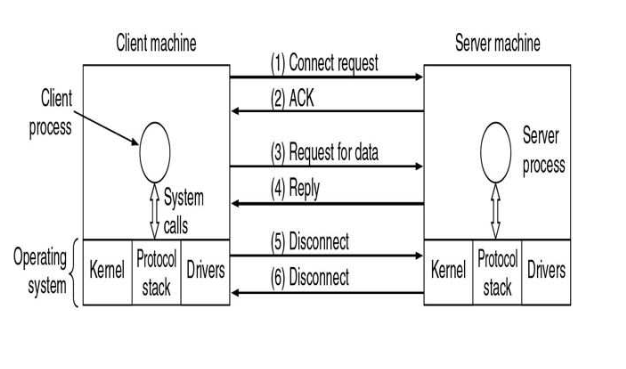
\includegraphics[width=\linewidth]{network-example.png}
  \caption{An example computer network interaction.}
  \label{fig:network-example}
\end{figure}
\subsection{Differentiating Factors of Networks}
One transmission type is \textbf{broadcast links}; broadcast networks have 
a single communication channel shared by all machine on a network. Packets
sent by any machine are received and an address field on the packet specifies
the intended recipient. Broadcasting is a mode of operation which allows a 
packet to be transmitted that every machine must process and multi-casting allows
a subset of machines to process a given packet. Another transmission type is
using \textbf{point-to-point links}, whose network consist of many connections
between individual pairs of machines. Packets travelling from source to 
destination must visit intermediate machines to determine a route - often
multiple routes of variant efficiencies are available and therefore optimization
is needed. \textbf{Unicasting} is used where point-to-point networks with a 
single sender and receiver pair can exchange data.
\subsection{Local Area Networks}
These are distinguished by three factors:
\begin{itemize}
    \item \textbf{Size}: Worst-case transmission time can be predicted in advance
    \item \textbf{Transmission Technology}: Wired or wireless
    \item \textbf{Topology}:
        \begin{itemize}
            \item \textbf{Bus}: only a single machine on the network can 
            transmit at any time. It requires a negotiation mechanism to resolve
            transmission conflicts. Ethernet is the most common bus network.
            \item \textbf{Ring}: Each transmission bit is propagated 
            individually. It requires access control to resolve propagation
            queuing.
        \end{itemize}
\end{itemize}
\subsection{Wide Area Networks}
This has a large-scale geographical coverage and typically a single network
provider is used across the WAN. They feature multiple hosts, typically owned
by non-network providers. They also feature multiple sub-networks, including
different transmission types and a range of \emph{routing} and \emph{switching}
infrastructure. Typically used in companies, universities etc. and end systems
usually connect into an ethernet switch. There are several types of WANs:
\begin{itemize}
    \item System interconnection: which can use short-range radio, low bandwidth
    and other numerous technologies like infrared etc.
    \item Wireless LAN: which has longer range radio, moderate bandwidth,
    requires transmission and reception devices; 802.11 family is most common.
\end{itemize}
A \textbf{link} is a connection between two devices in the network and 
\textbf{bandwidth} is the maximum speed in which data can be transmitted on
a link. Data is transferred through the internet using:
\begin{itemize}
    \item \textbf{Circuit-Switching}: End-to-end resources reserved for the 
    session; requires initial setup to reserve the resources. It has 
    dedicated resources with reserved bandwidth and has no sharing.
    \item \textbf{Packet-Switching}: Data stream divided into packets. Packets
    from different users share network resources. Its pros include: different
    packets can take different routes, it allows for resource sharing and thus
    allows for better utilization of network resources. Its cons include: no
    performance guarantee, possible congestions and packets maybe lost. See 
    figure \ref{fig:packet-switch}.
\end{itemize}
\begin{figure}
  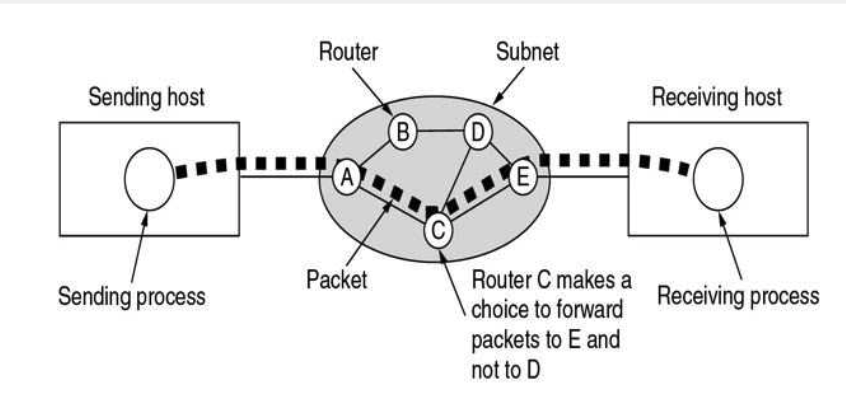
\includegraphics[width=\linewidth]{packet-switch.png}
  \caption{Packet switching on a network.}
  \label{fig:packet-switch}
\end{figure}
\subsection{Network Protocol Hierarchies}
The network can be considered as a stack of layers: each layer offers services
to the layers \emph{above it}. See figure \ref{fig:protocol-stack}.
\begin{figure}
  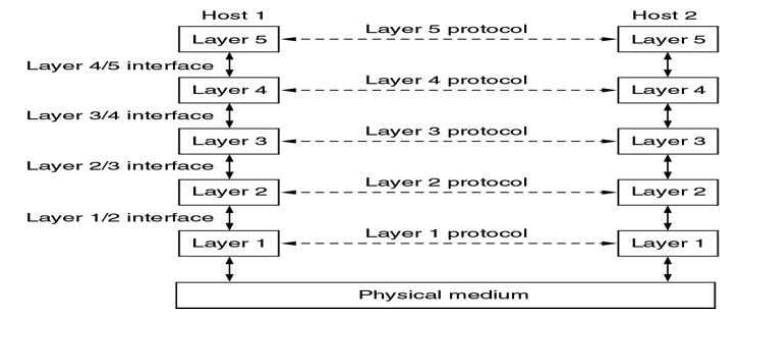
\includegraphics[width=\linewidth]{protocol-stack.png}
  \caption{Example protocol stack.}
  \label{fig:protocol-stack}
\end{figure}
There are different types of connections:
\begin{itemize}
    \item \textbf{Connection Oriented}: steps are \textbf{connect, use, disconnect}.
    Negotiation is inherent in connection setup; this is similar to a 
    telephone service.
    \item \textbf{Connectionless}: steps are just \textbf{use}. The message is routed 
    through intermediate nodes; this is similar to a postal service.
\end{itemize}
A \textbf{service} is a set of primitives that a layer provides to a layer above
it i.e. an interface between layers. A \textbf{protocol} is a set of rules
which govern the format and meaning of packets that are exchanged by peers 
within a layer i.e. packets sent between peer entities. Now we need a 
\textbf{network reference model}. Why? Because it provides a common baseline
for the development of many services and protocols by independent parties.
\subsection{OSI Reference Model}
The \textbf{open systems interconnection}, or OSI, is a reference model that 
states:
\begin{itemize}
    \item A layer should be created where a different abstraction is needed
    \item Each layer should perform a well-defined function
    \item The function of each layer should be chosen with a view toward
    defining internationally standardized protocols
    \item The layer boundaries should be chosen to minimize the information
    flow across the interfaces
    \item The number of layers should be large enough that distinct functions
    need not be thrown together in the same layer out of necessity, and 
    small enough that the architecture doesn't become unwieldy
\end{itemize}
The model is shown in figure \ref{fig:osi-model} and the TCP/IP model is shown
in figure \ref{fig:tcp-ip}.
\begin{figure}
  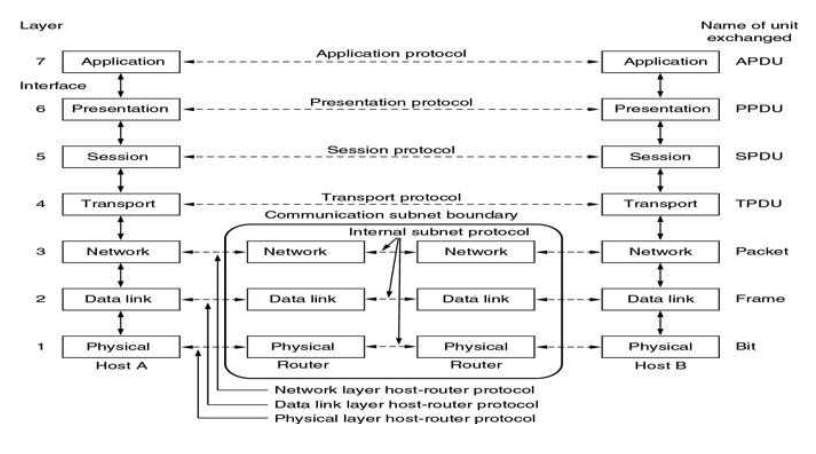
\includegraphics[width=\linewidth]{osi-model.png}
  \caption{The OSI model.}
  \label{fig:osi-model}
\end{figure}
\begin{figure}
  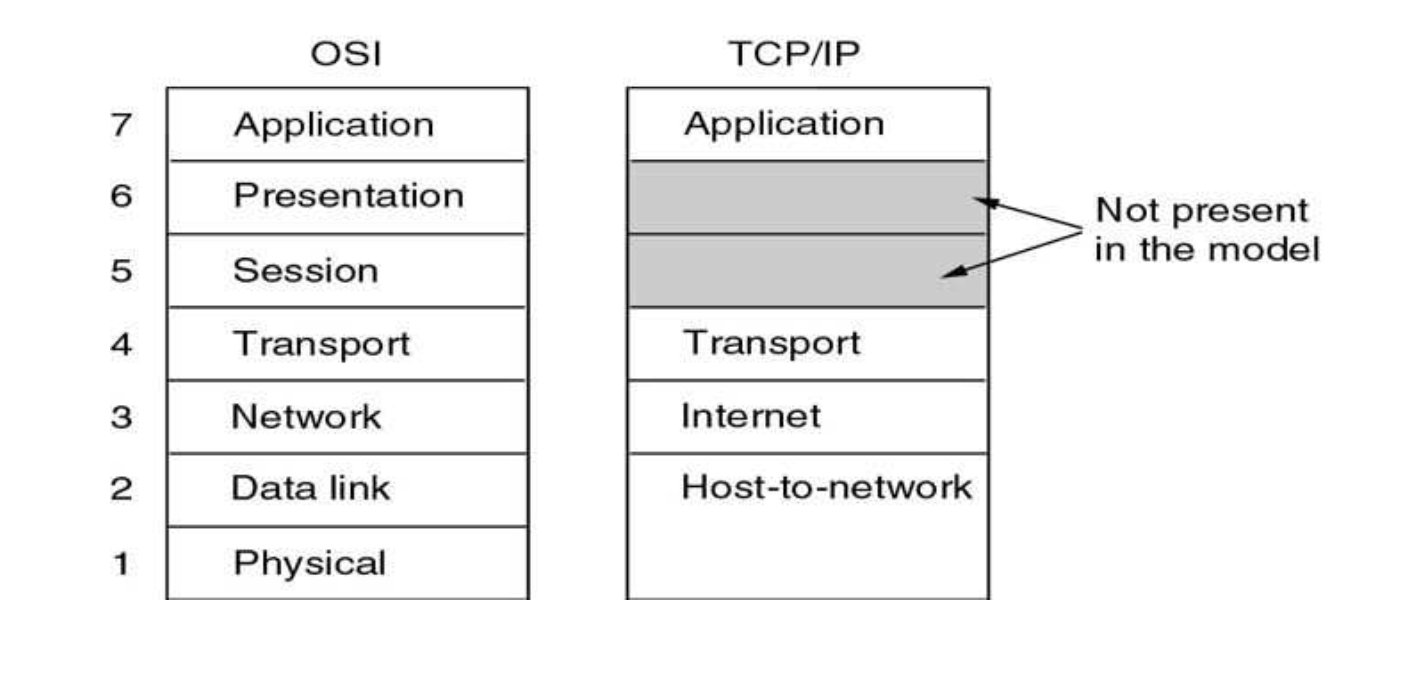
\includegraphics[width=\linewidth]{tcp-ip.png}
  \caption{The TCP/IP model.}
  \label{fig:tcp-ip}
\end{figure}
\subsection{Network Layers}
The \textbf{physical layer} corresponds to the signaling technology used.\\

Next, the \textbf{data link layer} has: frame management which takes packets from 
the network layers and encapsulates them into frames by adding a header, 
payload, trailer etc; ethernet device address and a MAC address which is a 
48-bit unique address and the data link layer's protocol specifies this 
address in the header.\\

The \textbf{network layer} has the primary function of
providing functionality to ``combine networks'' and route data through traffic.
It also creates an internet address space where each host has a 32-bit IP address,
runs IP routing software, implements packet routing across the network, defines 
a packet with a header containing information like packet size, source and 
destination address and the packet payload. Routers are used to transfer data
forward to nodes not directly connected to the network. Intermediate hosts are 
typically called \textbf{gateways}. MAC addresses are flat and portable while 
IP addresses are hierarchical and not portable and depend on the IP subnet to
which the node is attached. It basically provides service to the transport 
layer i.e. between nodes and hides details of link technology.
\begin{figure}
  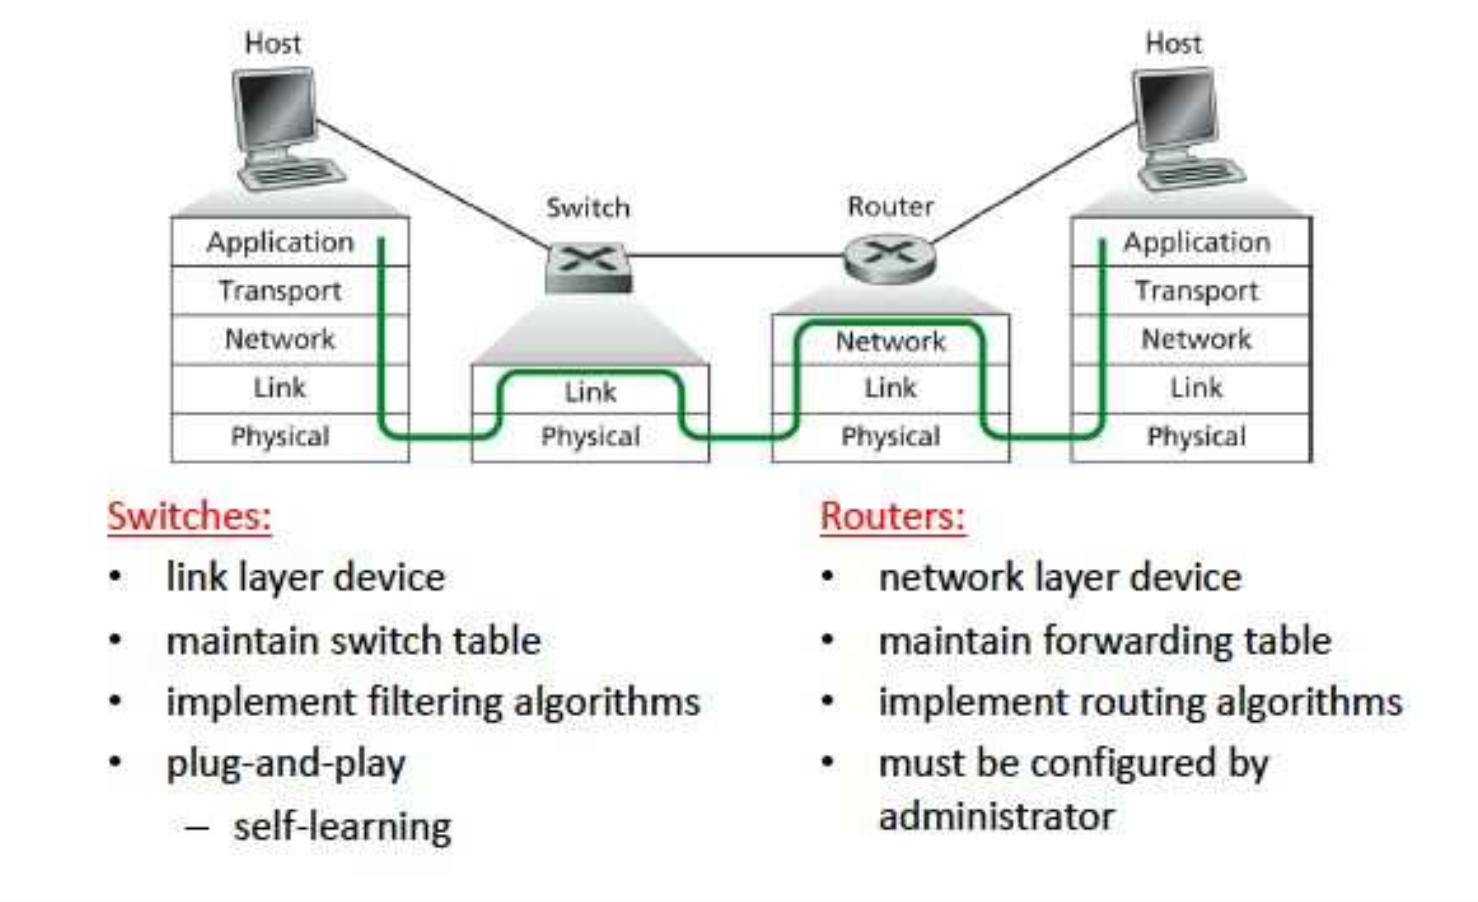
\includegraphics[width=\linewidth]{switches-routers.png}
  \caption{Switches and routers.}
  \label{fig:switches-routers}
\end{figure}
\\

The \textbf{transport layer} has two primary protocols:
\begin{itemize}
    \item \textbf{Transmission Control Protocol}: or TCP which is connection
    oriented and therefore has reliable delivery. It provides stream-oriented
    interface to applications.
    \item \textbf{User Datagram Protocol}: or UDP is connectionless and is 
    efficient but there is no guarantee of packet delivery.
\end{itemize}
This layer also provides the use of a 16-bit port number for applications. It
basically provides services to the application layer and relies on the network
layer for help and is a service between processes using sockets.\\

Examples of the \textbf{application layer} include: HTTP, FTP, SMTP, DNS etc.
It treats the layers below it as black boxes.

\section{Socket Programming}
Learning outcomes:
\begin{itemize}
    \item The use of sockets in network programming
    \item Difference between TCP and IP sockets and stream vs. datagram 
    sockets
    \item Socket system calls like: \texttt{socket(), bind(), accept()} and
    reading and writing
    \item Implement client and server programs
    \item How to write a server that which uses TCP sockets and can handle
    concurrent requests
\end{itemize}
\subsection{Port Numbers}
Popular applications like web and e-mail have well-known ports. Servers usually
have well-known port (0 - 1023) and clients pick an unused ephemeral port
(1024 - 65535). To uniquely identify traffic a 5-tuple is used which has
two IP addresses and a two port numbers and also the underlying transport
protocol. Code for an interaction is shown in figures \ref{fig:sock1} and
\ref{fig:sock2}.
\begin{figure}
  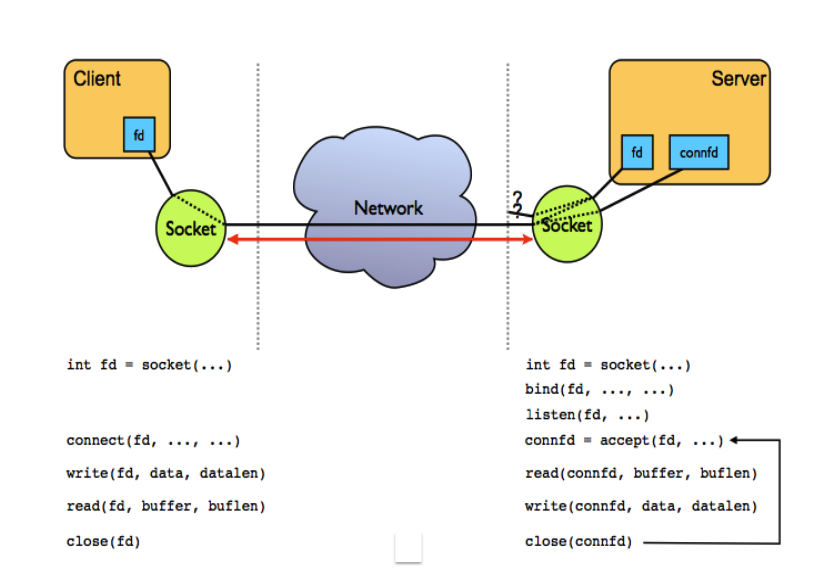
\includegraphics[width=\linewidth]{sock1.png}
  \caption{Communicating using a socket.}
  \label{fig:sock1}
\end{figure}
\begin{figure}
  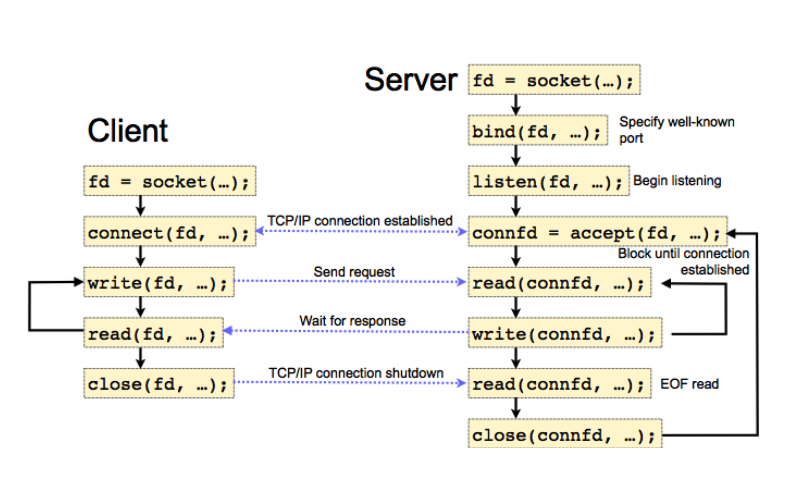
\includegraphics[width=\linewidth]{sock2.png}
  \caption{Code used for an interaction between a server and a client.}
  \label{fig:sock2}
\end{figure}
\subsection{Sockets}
Unbound sockets can be created which aren't connected to a the network and can 
be used as either a client or a sever. See figure \ref{fig:create-socket}.
\begin{figure}
  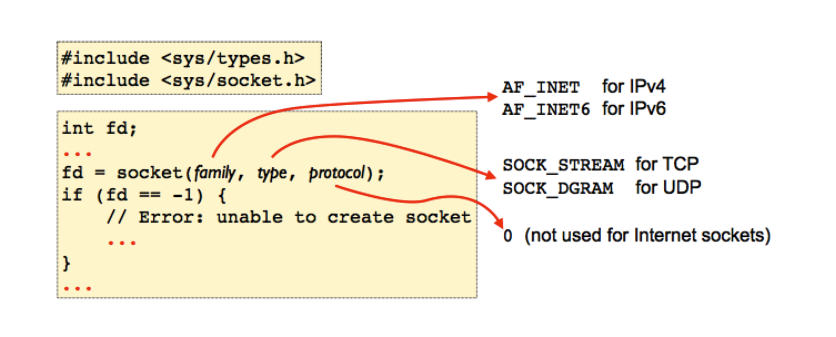
\includegraphics[width=\linewidth]{create-socket.png}
  \caption{Creating a socket in C.}
  \label{fig:create-socket}
\end{figure}
Once created, a socket can be bound to an internet port. A server process must 
assign an address to its socket and make it known to its clients. A client 
process may be able to obtain the correct socket address of any server on 
any host. The code is:
\begin{lstlisting}
    #include <sys/types.h>
    #include <sys/socket.h>

    if (bind(fd, addr, addrlen) == -1)
    {
        // Error 
        ...
    }
\end{lstlisting}
\textbf{Listening} for connections can be done on a socket so it ``listens'' 
for new connections. The backlog is the maximum number of connections the 
socket will queue up. The code is:
\begin{lstlisting}
    #include <sys/types.h>
    #include <sys/socket.h>

    if (listen(fd, backlog) == -1)
    {
        // Error
        ...
    }
\end{lstlisting}
We must remember to specify the port and the address when we call \texttt{bind()}
and \texttt{connect()}. The address can be either IPv4 or IPv6. Addresses 
are defined via struct \texttt{sockaddr}. It has a data field big enough
to hold the largest address of any family and \texttt{sa\_len} and \texttt{sa\_family}
can be used to set length and type of the address. It treats the address as
an opaque binary. It is defined as:
\begin{lstlisting}
    struct sockaddr {
        uint8_t sa_len;
        sa_family_t sa_family;
        char sa_data[22];
    };
\end{lstlisting}
Two variations exist for IPv4 and IPv6, \texttt{sockaddr\_in} can be used to 
store IPv4. It has the same size and memory layout as \texttt{sockaddr} but 
interprets the bits differently. The code is:
\begin{lstlisting}
    struct in_addr {
        in_addr_t s_addr;
    };

    struct sockaddr_in {
        uint8_t sin_len;
        sa_family_t sin_family;
        in_port_t sin_port;
        struct in_addr sin_addr;
        char sin_pad[16];
    };
\end{lstlisting}
Addresses can be created as:
\begin{lstlisting}
    #include <sys/types.h>
    #include <sys/socket.h>
    #include <netinet/in.h>
    #include <arpa/inet.h>

    struct sockaddr_in addr;
    ...
    addr.sin_addr.s_addr = INADDR_ANY;
    addr.sin_family = AF_INET;
    addr.sin_port = htons(80); // used to convert port

    if (bind(fd, (struct sockaddr *)&addr, sizeof(addr)) == -1) {
        ...
    }
\end{lstlisting}
\subsection{Byte Order}
Hosts differ on how they store data. In \textbf{little endian} the low-order
byte is stored at the lower memory location: \([b_0, b_1,...,b_n]\). It is 
used commonly in Intel's x86's. \textbf{Big endian} order has the high-order
byte stored at the lowest memory location: \([b_n, b_{n-1},...,b_0]\). Figure 
\ref{fig:endian} illustrates this point.
\begin{figure}
  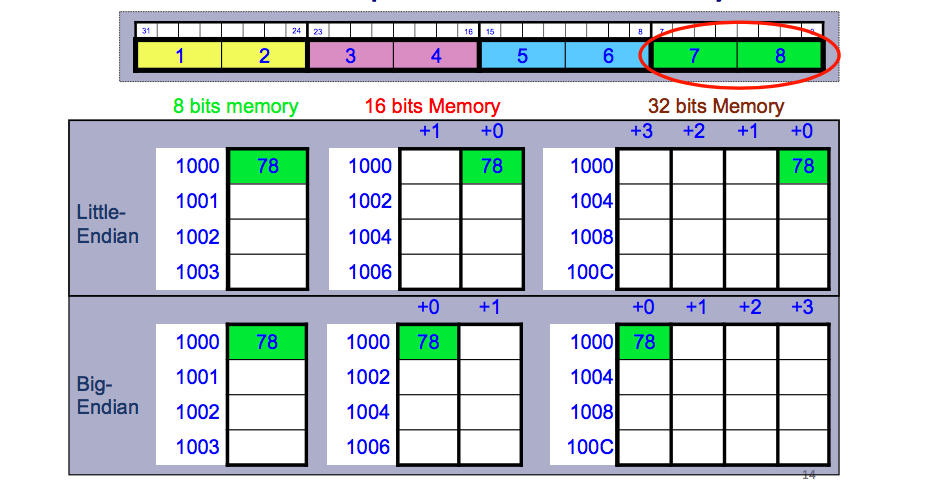
\includegraphics[width=\linewidth]{endian.png}
  \caption{Endian example.}
  \label{fig:endian}
\end{figure}
IP is big endian i.e. ``network byte order''. Therefore, to write portable code
we need to use \texttt{htons()} and \texttt{htonl()} to convert to network
byte order and use \texttt{ntohs()} and \texttt{ntohl()} to convert to host 
order. Doing so hides the details of the kind of machine being used. We us
system calls when sending/receiving data structures longer than one byte.
\subsection{Connections}
Connections can be accepted using the following code which returns the new file
descriptor for the connection and the client address:
\begin{lstlisting}
    int connfd;
    struct sockaddr_in cliaddr;
    socklen_t cliaddrlen = sizeof(cliaddr);
    ...
    connfd = accept(fd, (struct sockaddr *)&cliaddr, & cliaddrlen);
    // Error when connfd == -1
\end{lstlisting}
A TCP/IP server may have multiple connections outstanding, since only one
connection can be accepted at a time, we can accept connections and start a 
new thread for each. Note that each call to \texttt{accept()} returns a 
new file descriptor. A client can connect to a server using:
\begin{lstlisting}
    #include <netdb.h>

    // Note the definition of the hostnet struct
    struct hostnet {
        char* hname; // official host name
        char* h_alieases;
        int h_addrtype; // host address type
        int h_length; // lenght of address
        char** h_addr_list;
    }

    // translating server's name to an address
    struct hostnet* gethostbyname(char* name);
\end{lstlisting}
The code shown in figure \ref{fig:server-connect} tries to open a connection
to the server and times out after \(t\) seconds if no response.
\begin{figure}
  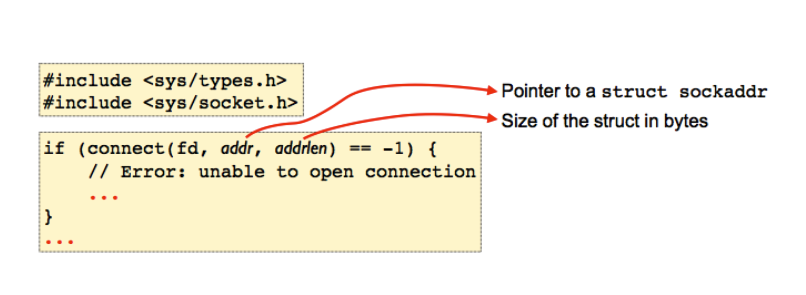
\includegraphics[width=\linewidth]{server-connect.png}
  \caption{Connecting to a server.}
  \label{fig:server-connect}
\end{figure}
The following code reads up to \texttt{BUFLEN} bytes of data from the connection
and blocks until data available. It returns the actual number of bytes read;
-1 otherwise. The data is \emph{not} null-terminated.
\begin{lstlisting}
    #define BUFLEN 1500
    ...
    ssize_t i;
    ssize_t rcount;
    char buf[BUFLEN];
    ...
    rcount = read(fd, buf, BUFLEN);
    if (rcount = -1) {
        // Error
        ...
    }
    for (i = 0; i < rcount; i++) {
        fprintf(stdout, "%c", buf[i]);
    }
    ...
    // Send data on a TCP/IP connection and blocks until all data can be
    // written 
    char data[] = "Hello";
    int datalen = strlen(data);
    ...
    if (write(fd, data, datalen) == -1) {
        // Error
        ...
    }
    ...
    // Close and destroy a socket
    // Close the file descriptor for each connection, then the file
    // descriptor for the underlying socket
    close(fd);
\end{lstlisting}
\subsection{Socket API}
This has data structures to store/convert information about hosts and 
connections: \texttt{gethostbyname, inet\_ntop, inet\_aton}. It has functions
to create and bind socket descriptors: \texttt{socket, bind, listen}. It also 
has functions to establish and tear down connections: \texttt{connect, accpet,
close, shutdown}. It has functions to send/receive data: \texttt{send, 
sendto, write, recv, recvfrom, read}.
\begin{itemize}
    \item \textbf{Stream sockets} are abstracted as sending a long stream of 
    characters and are typically implemented on top of TCP. Shown in figure
    \ref{fig:stream-socket}.
    \item \textbf{Datagram sockets} are abstracted as sending a single packet
    and are typically implemented on top of UDP. Shown in figure \ref{fig:datagram-socket}.
\end{itemize}
\begin{figure}
  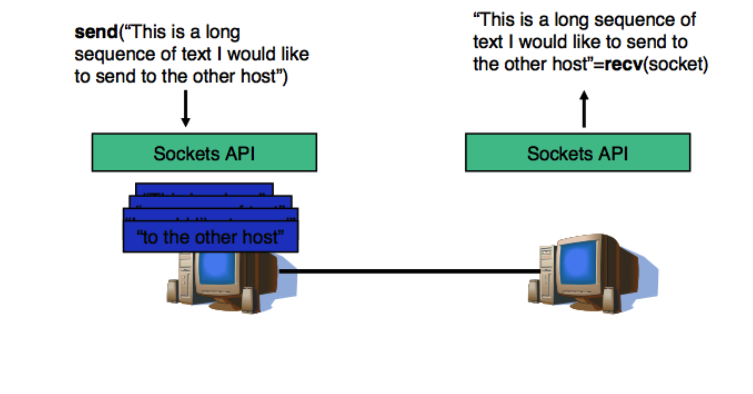
\includegraphics[width=\linewidth]{stream-socket.png}
  \caption{Stream socket.}
  \label{fig:stream-socket}
\end{figure}
\begin{figure}
  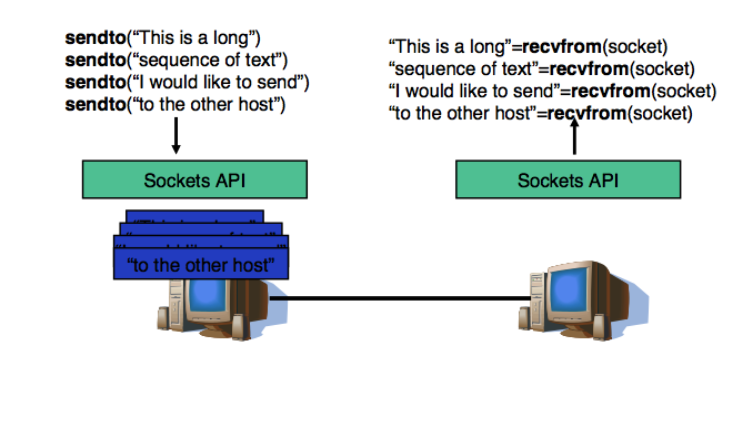
\includegraphics[width=\linewidth]{datagram-socket.png}
  \caption{Datagram socket.}
  \label{fig:datagram-socket}
\end{figure}
Read/write to a stream in TCP or a ``connected'' datagram UDP socket:
\begin{lstlisting}
    int read (in sockfd, char* buf, size_t nbytes);

    int write (in sockfd, char* buf, size_t nbytes);
\end{lstlisting}
The UDP \texttt{sendto()} and \texttt{recvfrom()} are defined as:
\begin{lstlisting}
    int sendto(int sockfd, char* buf, size_t nbytes, int flags, 
    struct sockaddr* destaddr, int addrlen);

    int recvfrom (int sockfd, char* buf, size_t nbytes, int flags,
    struct sockaddr* srcaddr, int* addrlen);
\end{lstlisting}
This sends a datagram to another UDP socket and the other reads a datagram
from a UDP socket.\\

The following code can be called just before \texttt{bind()} and allows 
\texttt{bind()} to succeed despite the existence of existing connections in the
requested TCP port. Connections in limbo with cause \texttt{bind()} to fail.
\begin{lstlisting}
    int yes = 1;
    setsockopt (fd, SOL_SOCKET, SO_REUSEADDR, (char*) &yes, sizeof(yes));
\end{lstlisting}
\section{Security}
Learning outcomes:
\begin{itemize}
    \item Key terms related to network security
    \item Symmetric and public key cryptography
    \item Use of cryptographic hash functions
    \item Digital signatures and certificates
    \item The use of SSL/TLS
\end{itemize}
Key terms include:
\begin{itemize}
    \item \textbf{Confidentiality} means that only the receiver should be able to 
    ``understand'' the contents of the message.
    \item \textbf{Authentication} is when the sender and receiver want to 
    verify the identity of each other.
    \item We also want \textbf{message integrity} i.e. the sender and the 
    receiver want to ensure that the message is not altered during transit.
    \item \textbf{Eavesdropping} means to intercept message.
    \item \textbf{Message corruption} is caused by actively inserting messages
    into connections
    \item \textbf{Impersonation} happens when spoofs source address in the 
    packet
    \item \textbf{Hijacking} means to take over ongoing connections by removing
    sender or receiver
    \item \textbf{Denial of service} is when a service is being prevented from
    being used by others e.g. by overloading resources
\end{itemize}
\textbf{Encrypting} means to send messages that are secret to everyone but
the intended receiver; the sender has to hide messages for sending so that 
no one else can understand it. \textbf{Decrypting} is essentially the opposite
of encrypting, in that the receiver has to ``un-hide'' and recover the message.
Figure \ref{fig:sym-crypto} shows symmetric cryptography and figure 
\ref{fig:secret-key} shows secret-key cryptography where both sender and the
receiver have agreed on the secret key in advance.
\begin{figure}
  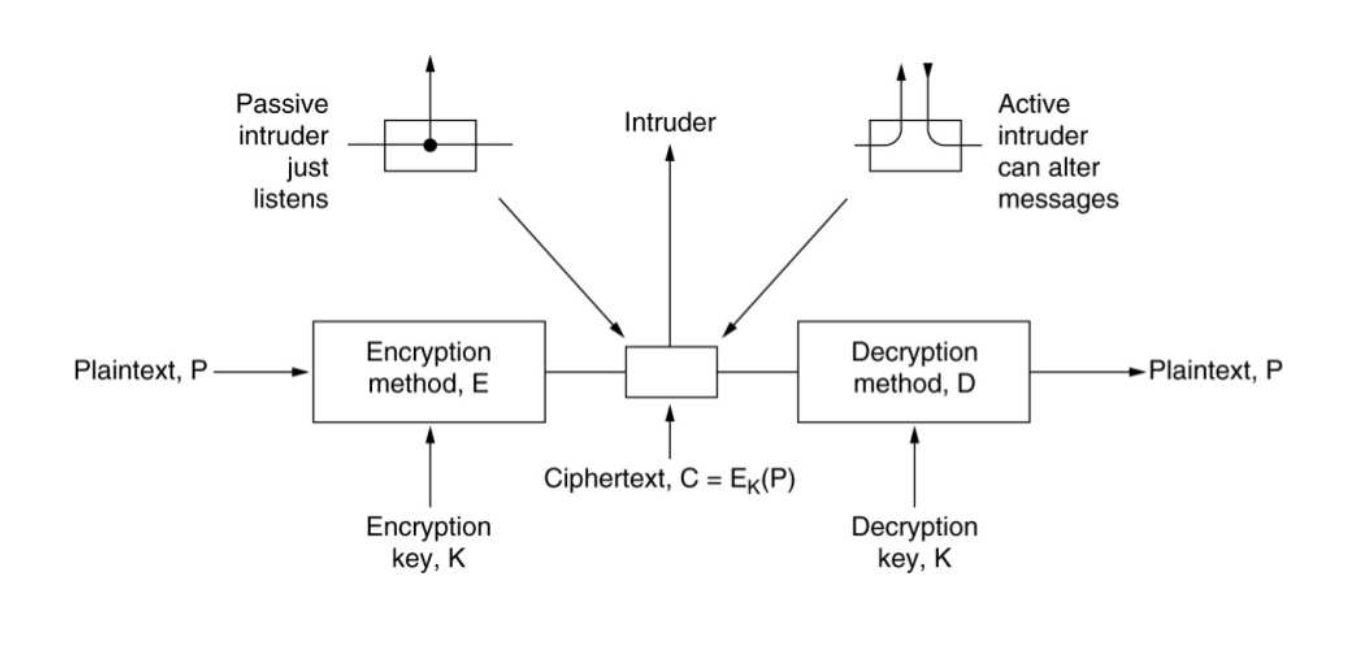
\includegraphics[width=\linewidth]{sym-crypto.png}
  \caption{Symmetric cryptography.}
  \label{fig:sym-crypto}
\end{figure}
\begin{figure}
  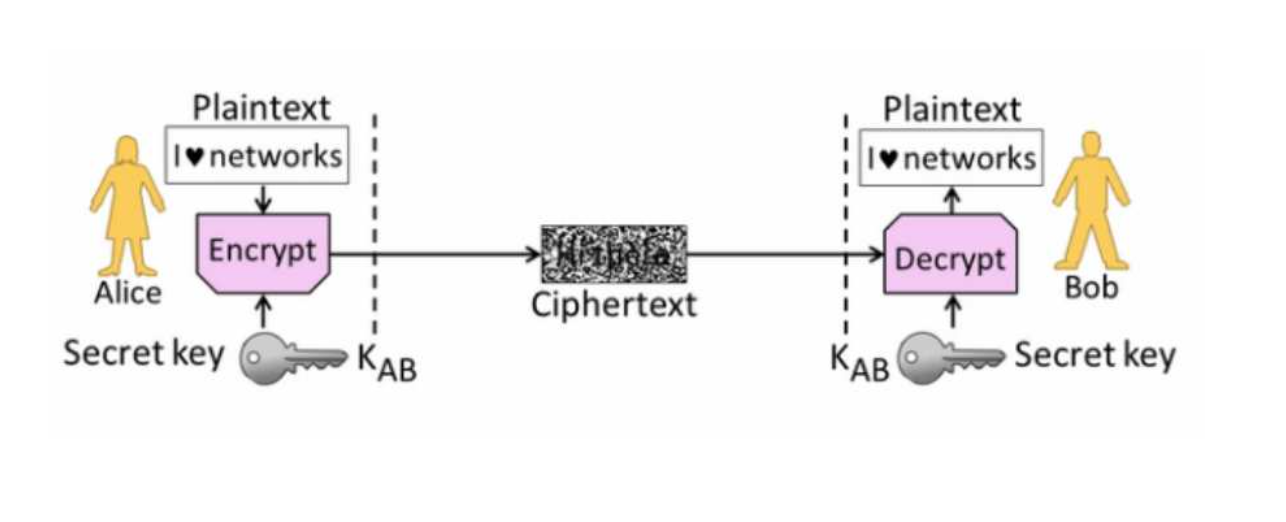
\includegraphics[width=\linewidth]{secret-key.png}
  \caption{Secret-Key cryptography.}
  \label{fig:secret-key}
\end{figure}
\subsection{Public-Key Cryptography}
The receiver generates two keys: a public key \(E\) for encrypting and a private
key \(D\) for decrypting. It publicizes \(E\) so people can use this for
encrypting and keeps \(D\) secret. The steps are:
\begin{itemize}
    \item The sender:
    \begin{itemize}
        \item Generates a secret key.
        \item Encrypts a message with the secret key.
        \item Encrypts the secret key with the receiver's public key.
        \item Sends the encrypted message and the encrypted key.
    \end{itemize}
    \item The receiver:
    \begin{itemize}
        \item Uses the private key to decrypt the secret key.
        \item Uses the secret key to decrypt the message.
    \end{itemize}
\end{itemize}
Summary of the symmetric and public-key cryptography:
\begin{center}
    \begin{tabular}{| l | l | l |}
    \hline \textbf{Property} & \textbf{Symmetric} & \textbf{Public Key} \\ \hline
    \hline Key Distribution & Hard - share secret per pair of users & Easier - publish public key per user \\ \hline
    \hline Runtime performance & Fast - good for high data rate & Slow - few, small, messages \\ \hline
    \end{tabular}
\end{center}
\subsection{Digital Signatures}
A digital signature is a mathematical link between a particular message and a 
particular public key. \(Sign(\)message, privateKey\()\) appends a string
of bits to a message and \(Verify(\)message, signature, publicKey\()\) 
allows the recipient to check that message. Without a public key, one cannot
forge/modify/sign a different message i.e. verification will fail. Figure
\ref{fig:signs} shows public-key signatures.
\begin{figure}
  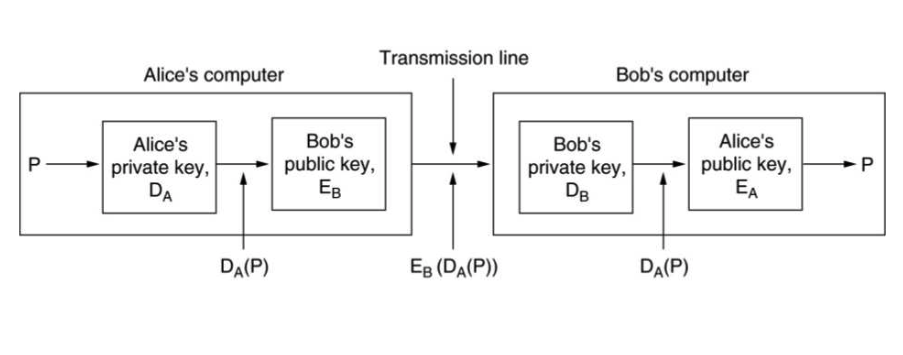
\includegraphics[width=\linewidth]{signs.png}
  \caption{Public-key signatures.}
  \label{fig:signs}
\end{figure}
Most digital signature algorithms (like RSA, DSA) hash a message before signing.
A hast algorithm takes a (possibly long) message and produces a fixed-length
digest (at least 160 bits). For crypto hashes, it should be infeasible to 
find two messages that hash to the same digest (called a ``collision''). The 
only problem now is how to obtain the correct public key of the receiver. A 
\textbf{certificate} is just a special kind of signed message where the message
says ``XYZ'' is the public key of a person plus some other data like a date. 
The signer is someone whose public key you already know. The primary job of
a certificate is to bind a public key to a user. Management of public keys 
is shown in figure \ref{fig:key-manage}.
\begin{figure}
  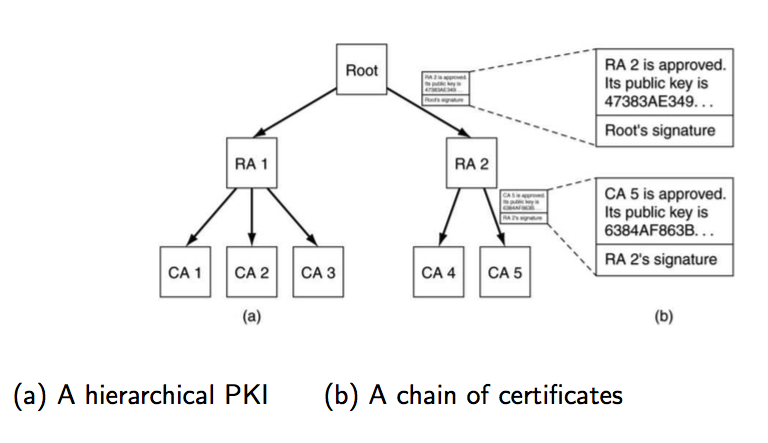
\includegraphics[width=\linewidth]{key-manage.png}
  \caption{Management of public keys.}
  \label{fig:key-manage}
\end{figure}
\subsection{SSL/TLS Secure Transmissions}
SSL/TLS is an almost-ubiquitous protocol for transmitting things securely over
the internet. It checks the certificate of the server you are talking to. It 
encrypts data and also authenticates it. The \textbf{Secure Sockets Layer} or
SSL provides transport layer security to any TCP-based application using SSL
services e.g. between web browsers, servers for e-commerce and also provides
security services such as server authentication, data encryption, client 
authentication. See figure \ref{fig:ssl} for the modification to the TCP 
structure.
\begin{figure}
  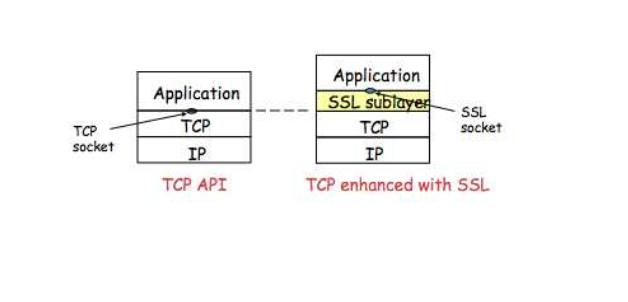
\includegraphics[width=\linewidth]{ssl.png}
  \caption{Secure sockets layer.}
  \label{fig:ssl}
\end{figure}
See figure \ref{fig:ssl-phases} for SSL phases. This first phase is the 
handshake where Bob establishes TCP connection to Alice; authenticates Alice
via CA-signed certificate and creates, encrypts (using Alice's public key),
sends master secret key to Alice. Alice and Bob use shared secrets to generate
four keys:
\begin{itemize}
    \item \(E_B\): Bob \(\rightarrow\) Alice data encryption key
    \item \(E_A\): Alice \(\rightarrow\) Bob data encryption key
    \item \(M_B\): Bob \(\rightarrow\) Alice MAC key
    \item \(M_A\): Alice \(\rightarrow\) Bob MAC key
\end{itemize}
Figure \ref{fig:ssl-data-transfer} shows SSL data transfer.
\begin{figure}
  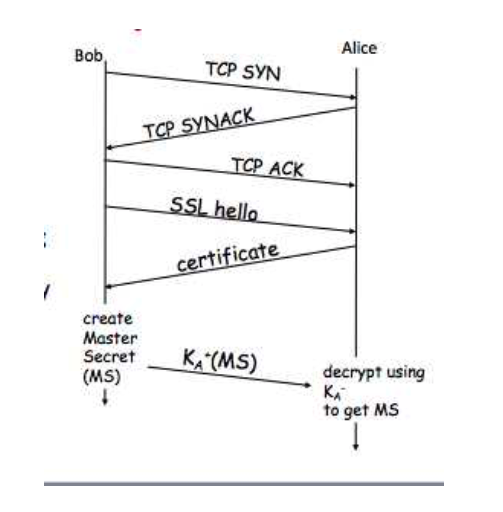
\includegraphics[width=\linewidth]{ssl-phases.png}
  \caption{SSL phases.}
  \label{fig:ssl-phases}
\end{figure}
\begin{figure}
  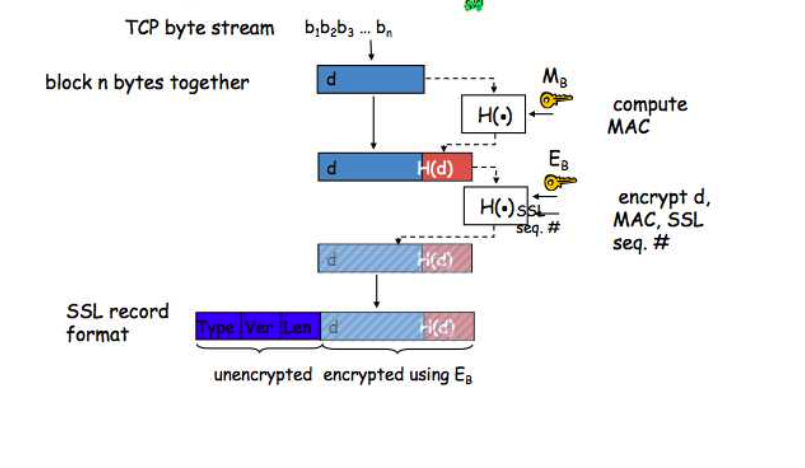
\includegraphics[width=\linewidth]{ssl-data-transfer.png}
  \caption{SSL data transfer.}
  \label{fig:ssl-data-transfer}
\end{figure}
\section{TCP/IP}
Learning outcomes:
\begin{itemize}
    \item Network layer protocols like IP addresses, subnets, routing,
    fragmentation
    \item Transport layer protocols i.e. TCP, UDP, TCP connection, congestion
    control
    \item Format and use of protocol headers and how Wireshark can be used
    \item ARP
\end{itemize}
Data traffic is divided into packets, each of which contains a header with 
source and destination address. The packets travel separately through the 
network. The sender puts data into packets. The network interface hardware
then transforms data for physical transmission. The network delivers packets
to a variable destination, possibly along different paths. The receiver 
converts physical signal back into a data packet and assembles packets back
into data. Note that some packets maybe lost, corrupted or delivered out of 
order; error detection or correction is provided by higher-level protocol. \\

In a \textbf{connectionless} transfer the datagrams are injected into subnet
independently and packets individually routed to destination. With the internet
the packets could move in a potentially unreliable subnet - QoS is not easily 
implemented. In a \textbf{connection-oriented} transfer packets travelling 
between destinations all use the same route. An example is a telecommunication
company which guarantees reliability as QoS is important. There are several 
issues to be considered when connecting networks such as: different network
types and protocols, different motivations for network choices and different
technologies at both hardware and software levels. Connectionless networks
can be connected using datagrams. See figure \ref{fig:internetworking} for 
internetworking and figure \ref{fig:network-diff} for how networks can differ.
\begin{figure}
  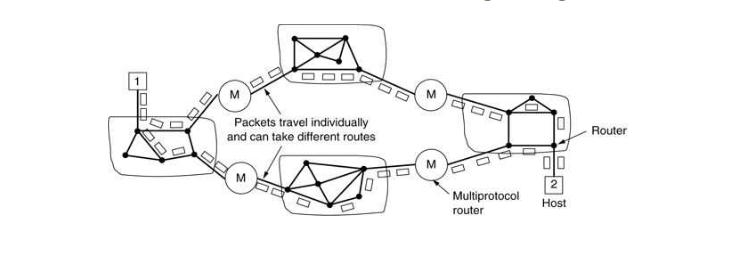
\includegraphics[width=\linewidth]{internetworking.png}
  \caption{Internetworking.}
  \label{fig:internetworking}
\end{figure}
\begin{figure}
  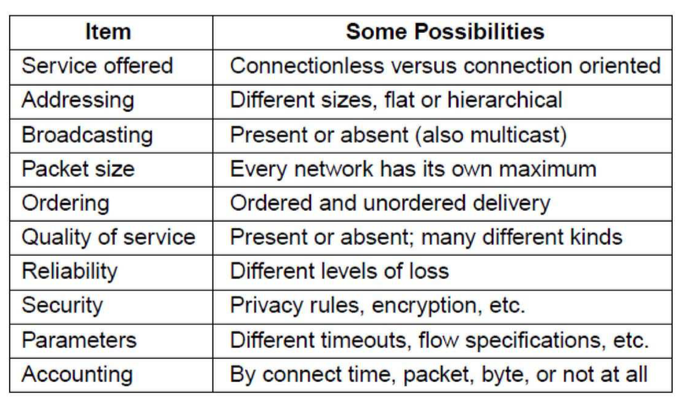
\includegraphics[width=\linewidth]{network-diff.png}
  \caption{How networks can differ.}
  \label{fig:network-diff}
\end{figure}
\subsection{Internet Protocol}
IP provides a ``best effort'' service to route datagrams from source host to 
destination host. These hosts may be on the same network or on different
networks. It uses a connectionless model; its design goals are:
\begin{itemize}
    \item Services should be independent of router technologies
    \item Transport layer should be shielded from number, type and topology of 
    routers
    \item Network addressing should use a uniform numbering plan
\end{itemize}
\subsection{IPv4 Frame Structure}
\begin{figure}
  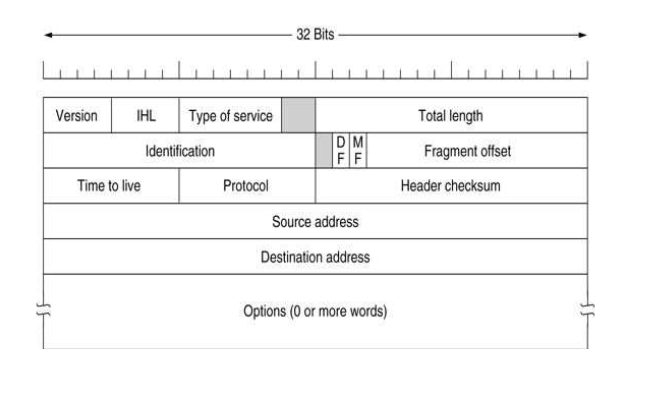
\includegraphics[width=\linewidth]{ipv4-header.png}
  \caption{IPv4 header showing frame structure.}
  \label{fig:ipv4-header}
\end{figure}
IPv4 frame consists of a header and some text. The header is a 20 byte fixed 
part + variable-length optional part. The version could be set as IPv4 or IPv6.
IHL is the header length and type differentiates different classes of service.
The total length is the header and payload, maximum length is 0xffff or 
65535 bytes. Identification allows host to determine which datagram the new 
fragment belongs to - all fragments of the same datagram have the same ID. 
DF is the don't fragment byte. MF is the more fragment byte i.e. are there more
or is this the last one? Fragment offset means where in the datagram the 
current fragment belongs. TTL limits packet lifetime; could be in hops or 
seconds. Protocol refers to TCP, UDP or others. The header checksum verifies
the header only. Finally, options include security, strict vs loose routing,
record route, timestamp etc.
\subsection{Fragmentation}
All networks have a maximum size for packets motivated by various factors like:
hardware, OS, protocols, standards compliance, desire to reduce transmissions 
due to errors, desire for efficiency in communication channel etc. 
\textbf{Fragmentation} is the division of packets into fragments, this allows
network gateways to meet constraints. Figure \ref{fig:frag} shows fragmentation
ranging from on constraints to an 8-byte constraint to a 5-byte constraint.
\begin{figure}
  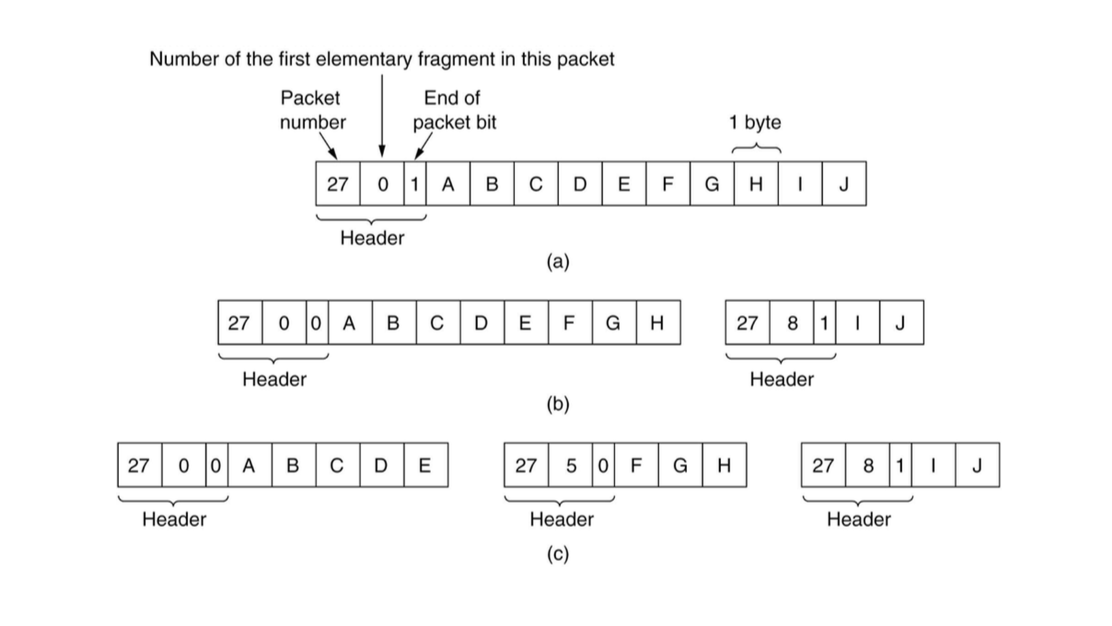
\includegraphics[width=\linewidth]{frag.png}
  \caption{Packet fragmentation.}
  \label{fig:frag}
\end{figure}
\subsection{IP Address}
An IP address is a 32-bit number that encodes network and host information. See
figure \ref{fig:ip-address.}
\begin{figure}
  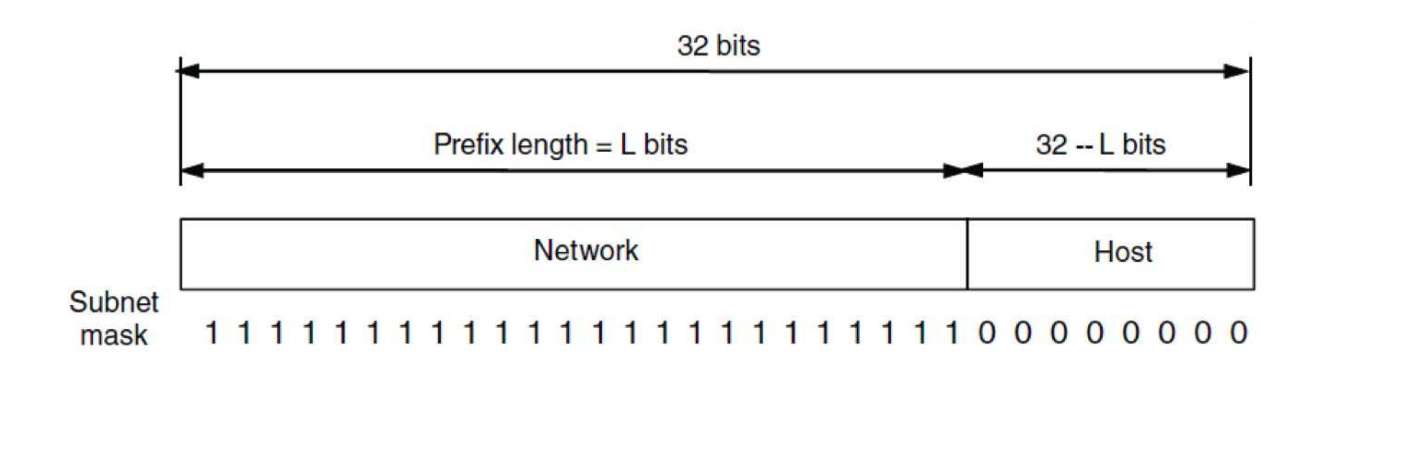
\includegraphics[width=\linewidth]{ip-address.png}
  \caption{IP address.}
  \label{fig:ip-address}
\end{figure}
\textbf{Subnetting} allows networks to be split into several parts for internal
use while appearing as a single network for external use. Prefixes are written
are as the lowest IP address in the block, followed by the size of the block.
The size of the block is written with a slash at the end followed by a number
indicating the number of bits in the network portion. Since IP addresses are 
getting scarce a NAT is used to allow for unique addresses within a network, 
but a shared IP address when it exits out of the local network. IPv6 is the 
solution to the scarcity of the IPv4 problem, and uses 128-bit addresses with
the goals to reduce routing table size, simplify protocol, improve security,
roaming host without changing address allow future protocol evolution. 
\textbf{Internet control protocols} control protocols int he network layer on
the internet; they are ICMP, ARP, RARP. The ICMP internet control message 
protocol is used for testing and monitoring ambient conditions between hosts
and routers; see \texttt{traceroute}. Types of messages used:
\begin{center}
    \begin{tabular}{| l | l |}
    \hline \textbf{Message type} & \textbf{Description} \\ \hline
    \hline Destination unreachable & Packet could not be delivered \\ \hline
    \hline Time exceeded & Time to live field hit 0 \\ \hline
    \hline Parameter problem & Invalid header field \\ \hline
    \hline Source quench & Choke packet \\ \hline
    \hline Redirect & Teach a router about geography \\ \hline
    \hline Echo and Echo reply & Check if a machine is alive \\ \hline
    \hline Timestamp request/reply & Same as Echo, but with timestamp \\ \hline
    \hline Router advertisement/solicitation & Find nearby router \\ \hline
    \end{tabular}
\end{center}
\subsection{Transport Layer}
The main function of this layer is to provide reliable, efficient data transfer
from source to destination, independent of the physical and data layers. The
transport layer \textbf{services} provide interfaces between the network and 
the application layer and the \textbf{entities}, which are the software and 
hardware that does the actual work, can exist in multiple locations.The services 
provide a logical connection between application processes running on different
hosts: connection establishment/release (for TCP only) and data transfer. 
Although the network and transport layers are similar, we need the transport 
layer as the it runs on hosts unlike the network layer which runs mostly on 
routers; it can also fix reliability issues on top of an unreliable network. 
Messages sent to and from the transport layer are abstracted further and are
called transport protocol data units, TPDUs. So we have encapsulation of TPDUs
in packets (from the network layer) in frames (from the data link layer). See
figure \ref{fig:encaps}.
\begin{figure}
  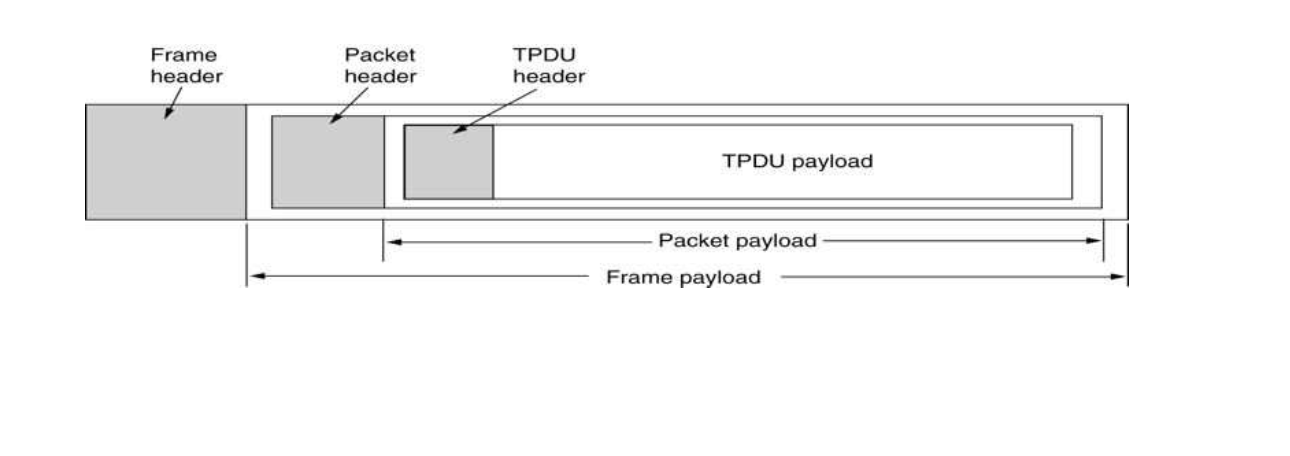
\includegraphics[width=\linewidth]{encaps.png}
  \caption{Encapsulation of messages.}
  \label{fig:encaps}
\end{figure}
\textbf{Primitives} are core functions which allow interface with transport 
services.
\begin{center}
    \begin{tabular}{| l | l | l |}
        \hline \textbf{Primitive} & \textbf{Packet sent} & \textbf{Meaning} \\ \hline
        \hline LISTEN & none & Block until some process tries to connect \\ \hline
        \hline CONNECT & CONNECTION REQ. & Actively attempt to establish a connection \\ \hline
        \hline SEND & DATA & Send information \\ \hline
        \hline RECEIVE & none & Block until a DATA packet arrives \\ \hline
        \hline DISCONNECT & DISCONNECTION REQ. & This side wants to release the connection \\ \hline
    \end{tabular}
\end{center}
\begin{figure}
  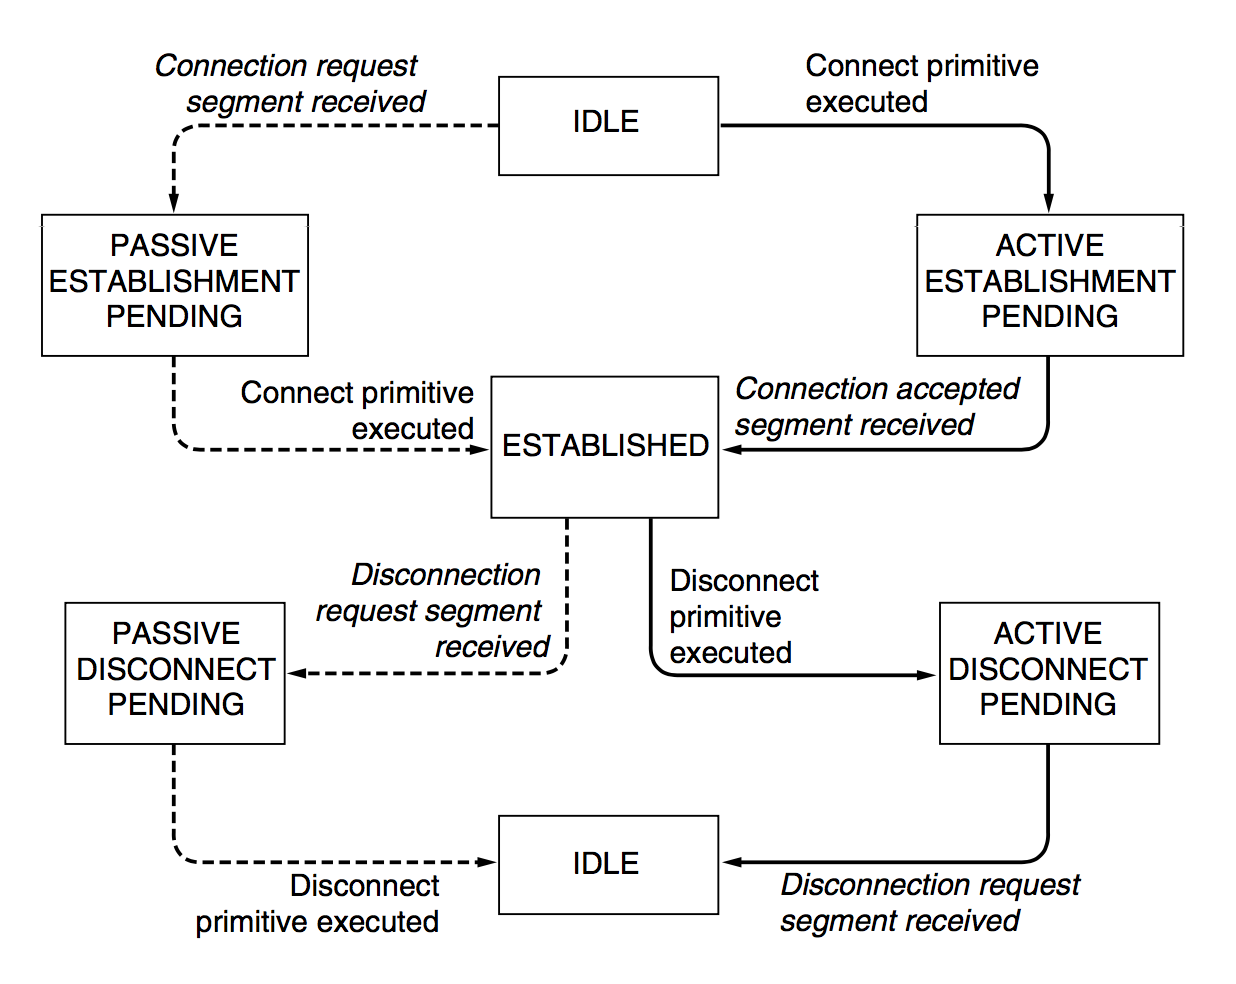
\includegraphics[width=\linewidth]{connection-state.png}
  \caption{The dashed lines show the server's state sequence and the solid lines
  show the client's state sequence. The text in italics is triggered after 
  packet arrival.}
  \label{fig:connection-state}
\end{figure}
Transport services are implemented as protocols used between transport entities.
Transport is similar to the data link layer as they both have error control,
sequencing and flow control; the differ in: physical network vs physical/data/
network, addressing, connection establishment and storage. \\

Specification of the remote process to ``connect to'' is required at both the
transport and the application layer. Addressing in the transport is usually 
done using port numbers. A process server intercepts inbound connections and 
spawns requested server and attaches the inbound connection. Addressing the
the network layer is done using IP addresses. Port number can range from 0 
to 65535 and split into three segments: well-known ports (0 - 1023), registered
ports (1024 - 49151) and dynamic ports (49152 - 65535).
\begin{figure}
  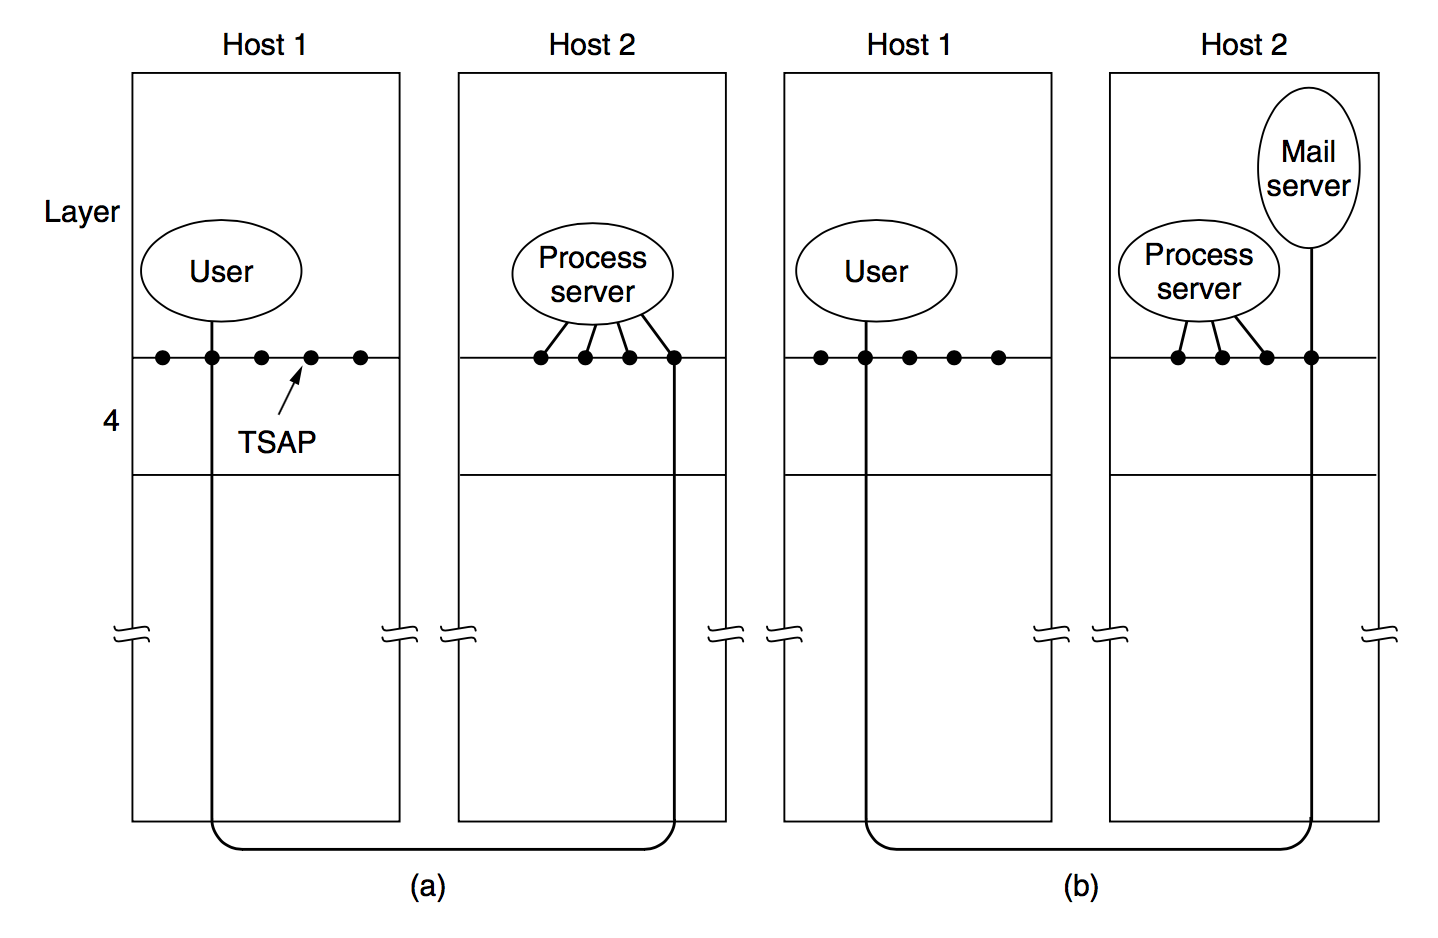
\includegraphics[width=\linewidth]{process-server.png}
  \caption{(a) shows process server interception and (b) shows how the process
  server goes back to listening after attaching the process.}
  \label{fig:process-server}
\end{figure}
Connections can lose, duplicate and store packets, complicating things. 
Congested networks can cause delayed acknowledgements incurring multiple 
repeated transmissions, any of which may arrive out of sequence i.e. delayed
duplicates. Therefore causing applications to degenerate with such congestions.
\subsection{UDP}
UDP transmits in segments consisting of a header followed by the payload. UDP
headers contain source and destination ports, payload is handed to the process
which is attached to the particular port at destination. The main advantage of
using this over raw IP is the ability to specify a source and destination. 
Note that both the source and destination are required - destination allows 
initial routing for incoming segments and source allows reply routing for
outgoing segments. It has advantage that it provides an IP interface with 
mutliplexing and de-mutliplexing and transmission efficiencies. It has the 
disadvantage of supporting flow control, error control and re-transmission of 
bad segments. Therefore, UDP is good when applications required precise 
control over packet flow, error and timing. See figure \ref{fig:udp-header}.
\begin{figure}
  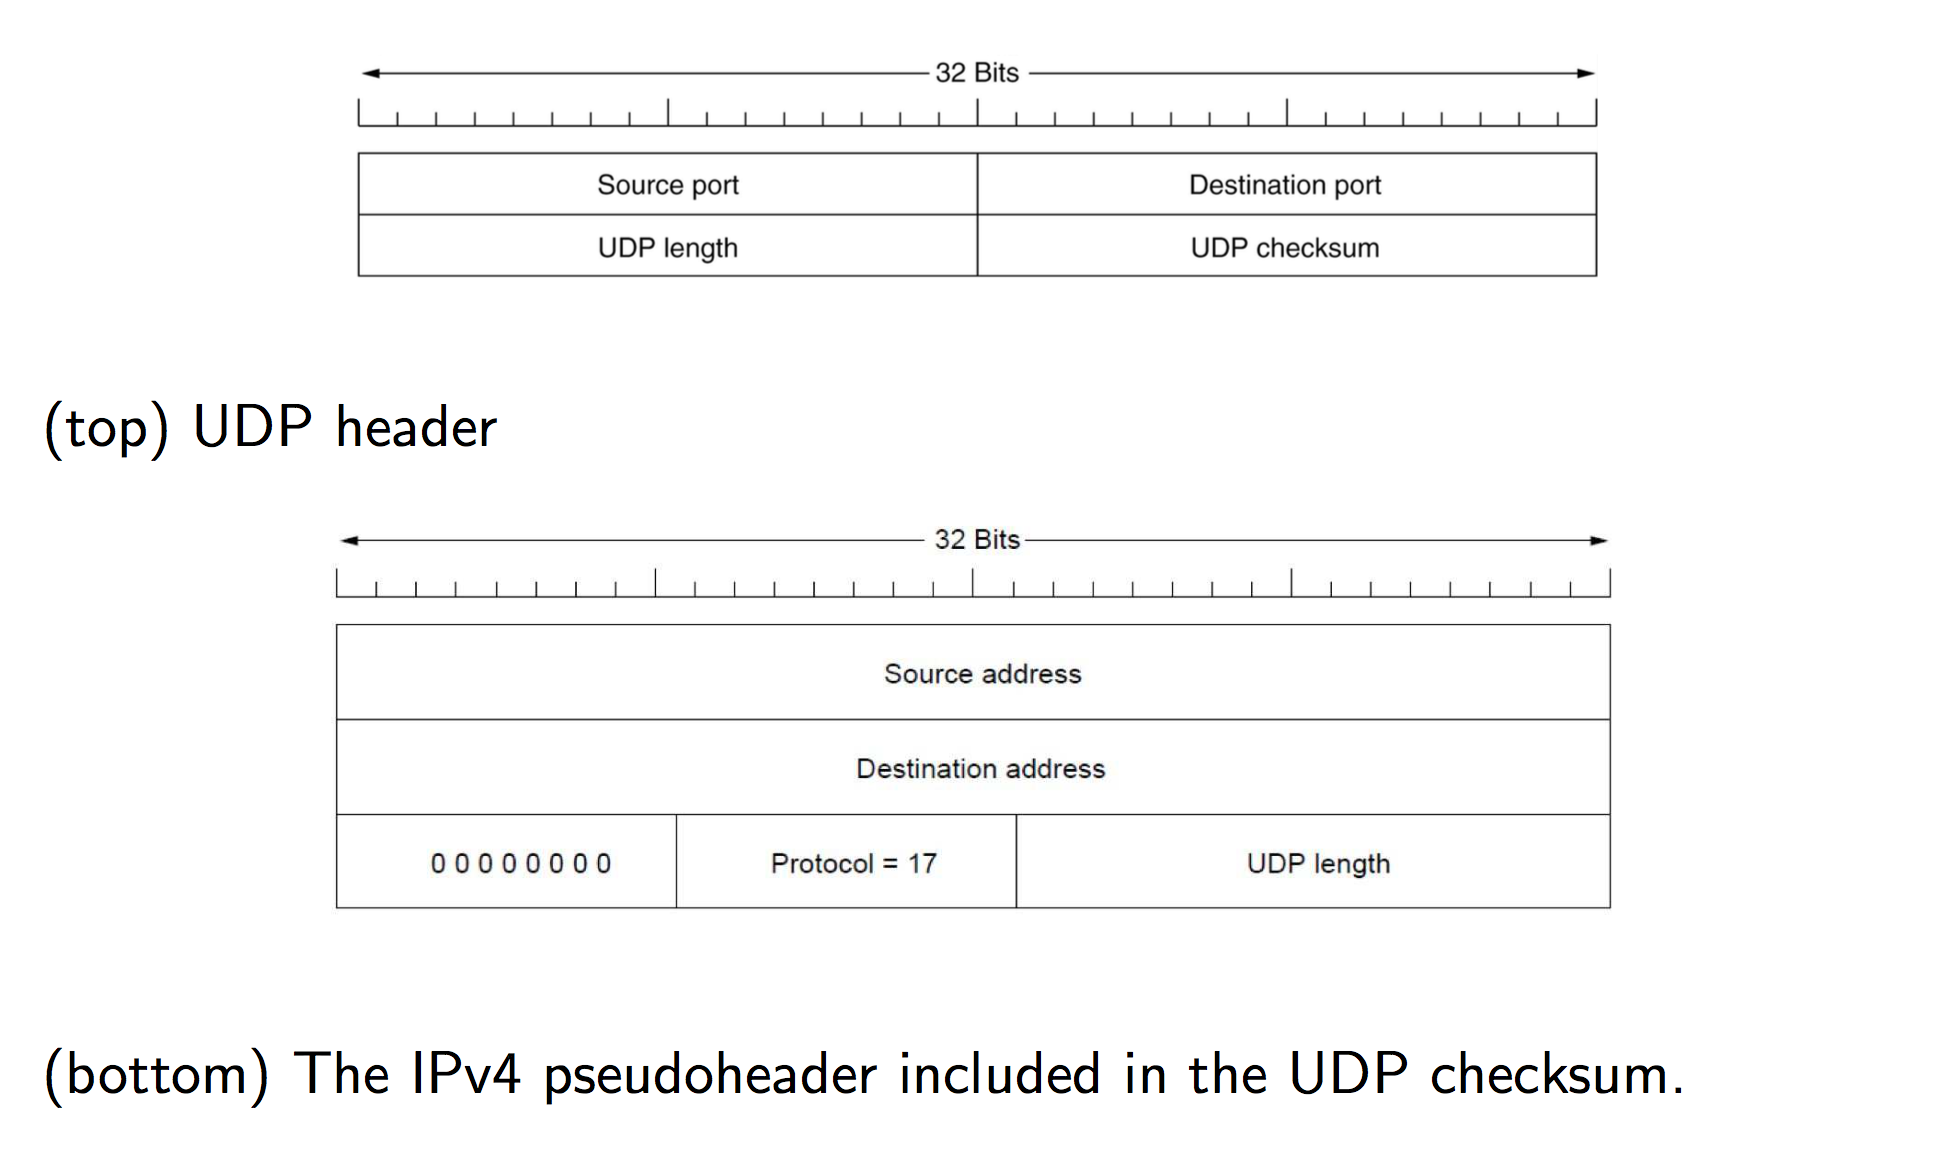
\includegraphics[width=\linewidth]{udp-header.png}
  \caption{The UDP header.}
  \label{fig:udp-header}
\end{figure}
\subsection{TCP}
The TCP transport entity manages TCP stream and interfaces to the IP layer. It
accepts user datagrams and segments them and sends each segment as a separate
IP datagram and the recipient TCP entities do the reconstruction. For the TCP
service to be activated, connections must be explicitly established between
a socket at the sending host and a socket of the receiving host.
\begin{figure}
  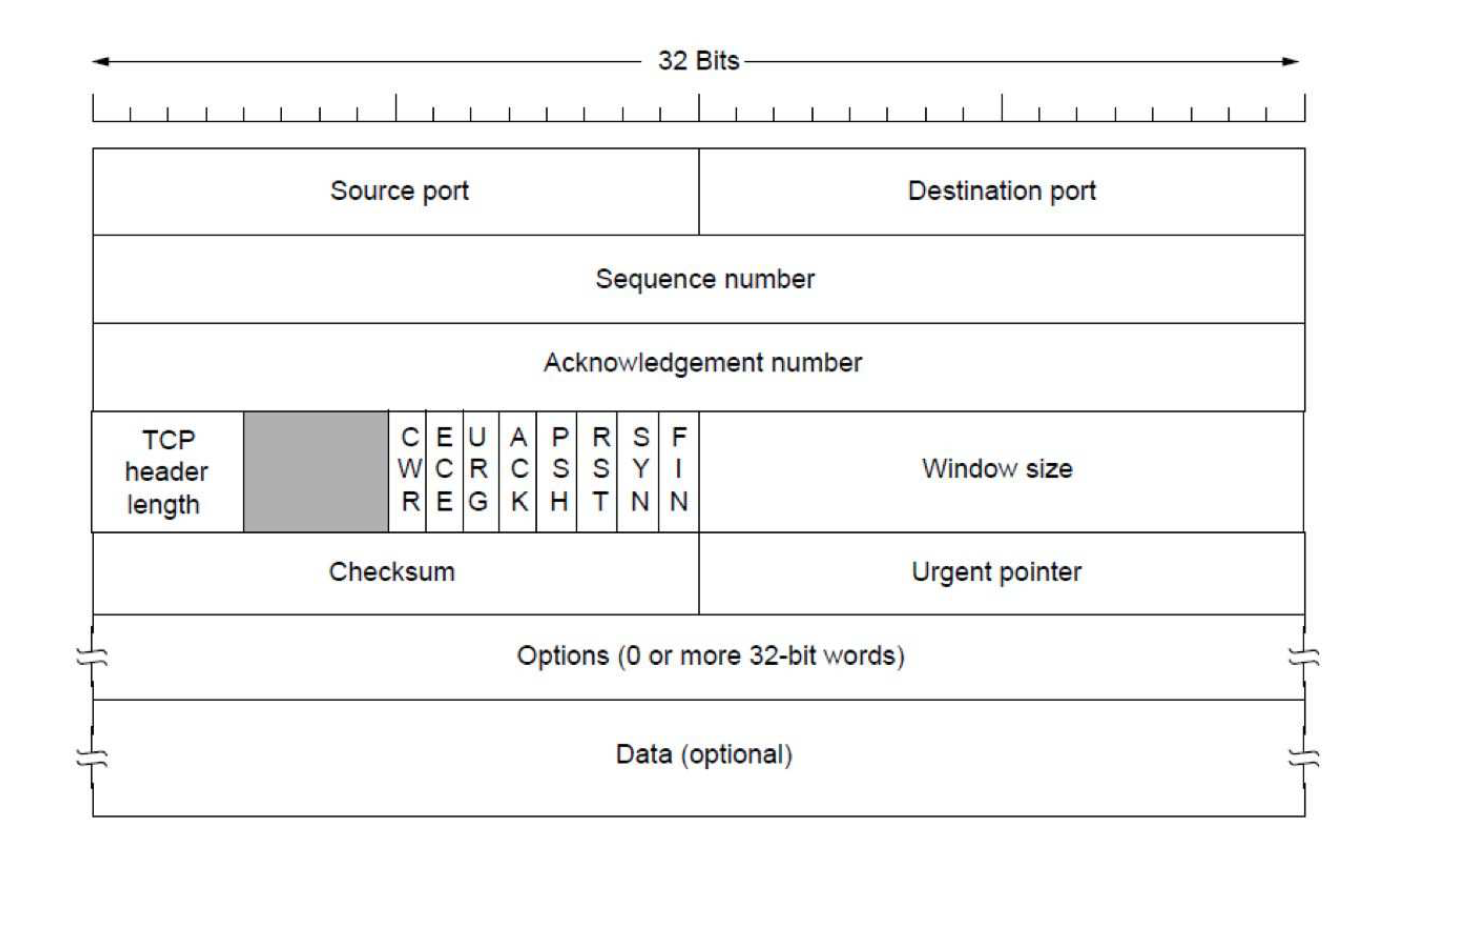
\includegraphics[width=\linewidth]{tcp-header.png}
  \caption{The TCP header.}
  \label{fig:tcp-header}
\end{figure}
\subsubsection{Feature of TCP Connections}
Features of TCP are:
\begin{itemize}
    \item Full duplex - data in both direction simultaneously
    \item Point to point - exact pairs of sender and receivers
    \item Byte streams, not message streams - message boundaries are not
    preserved
    \item Buffer capable - TCP entity can choose to buffer prior to sending; 
    the PUSH flag indicates a transmission must not be delayed; URGENT flag
    indicates that transmission should be send immediately.
\end{itemize}
\subsubsection{TCP Details}
The data exchanged between TCP entities is in segments with each segment 
having a 20-byte header and 0 or more bytes of data. TCP entities decide
on how long the fragments should be while following the constraints: 65515-byte
IP payload; Maximum Transfer Unit (MTU) - generally 1500 bytes. \textbf{Sliding
window protocol}: sender transmits and starts a timer; the receiver responds 
with an acknowledgement; if the timer runs out, the segment is sent again.
\subsubsection{Three-Way Handshake}
Goal of a reliable connection are: ensuring packet lifetimes are bounded, assign
sequence numbers that won't be used within the packet lifetime and ensure that 
initial start and respond number sequences are agreed at the start of connection
establishment. A three-way handshake is the solution to the problem where both
sides assign the same sequence of numbers e.g. after host/router crash. Sender 
and receiver agree on which sequencing strategy each will use before exchanging
TPDUs.
\begin{figure}
  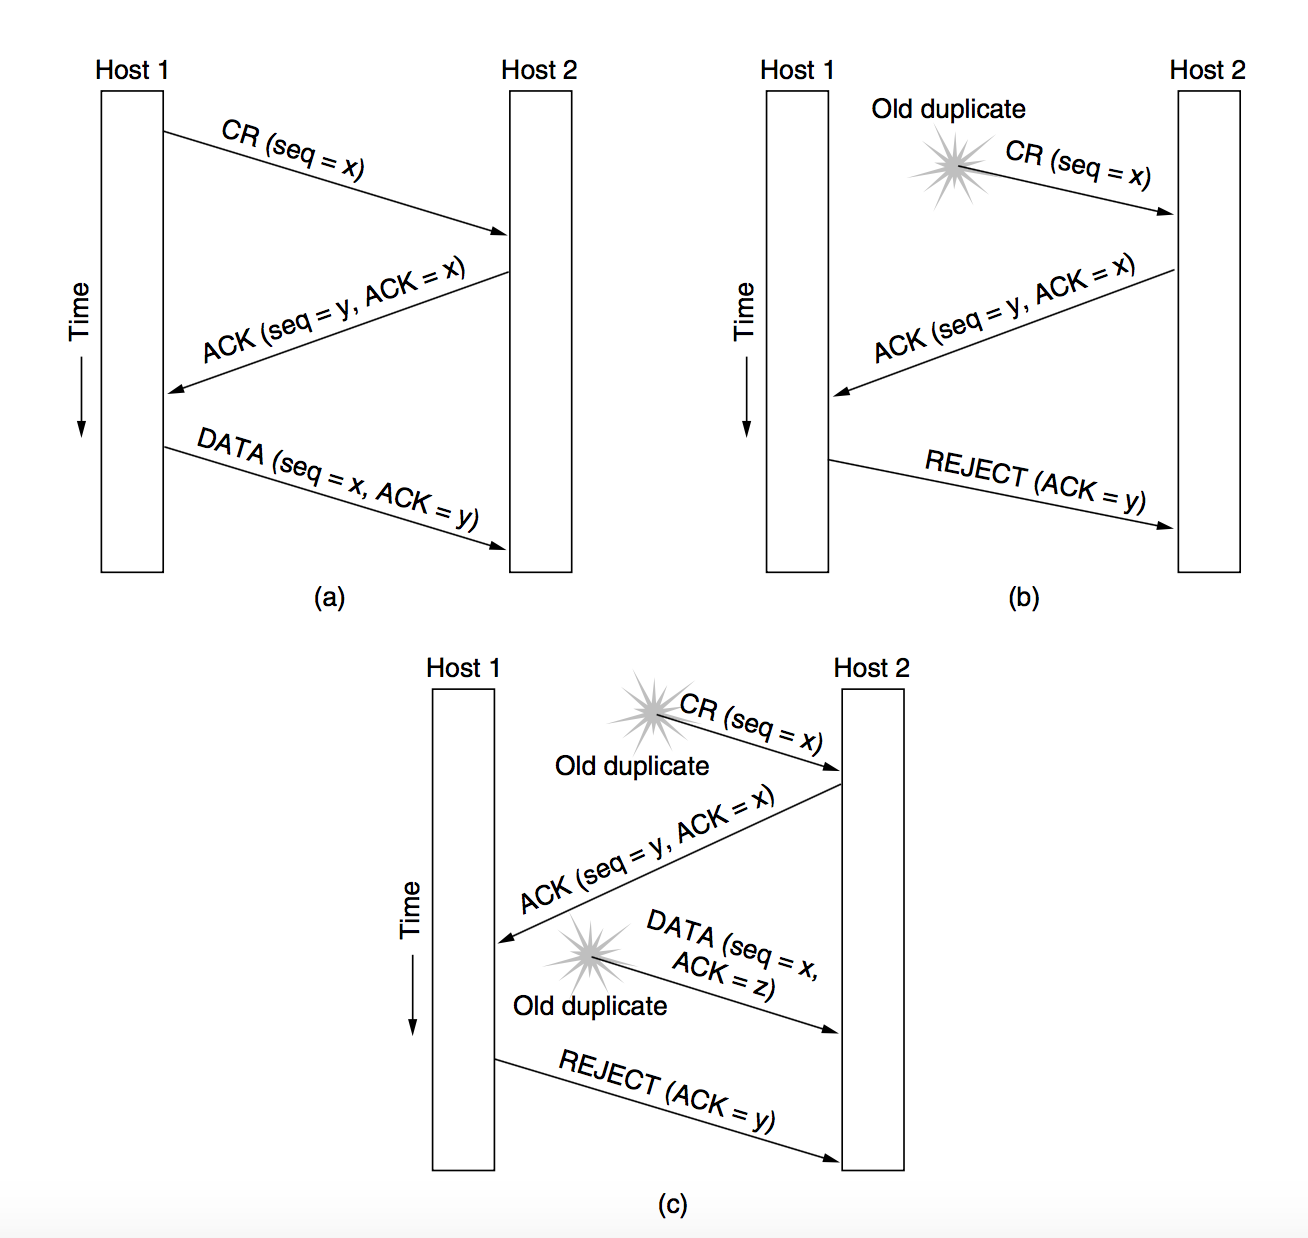
\includegraphics[width=\linewidth]{three-way-handshake.png}
  \caption{(a) Normal operation. (b) Old CONNECTION REQUEST appearing out of 
  nowhere. (c) Duplicate CONNECTION REQUEST and duplicate ACK.}
  \label{fig:three-way-handshake}
\end{figure}
\subsection{Congestion Control}
When networks are overloaded, congestion occurs, potentially affecting all 
layers. Although lower layers like physical and data link, try to fix this,
in reality TCP impacts congestion most significantly as it offers methods to 
transparently reduce the data rate and hence, reduce congestion. TCP adopts
a defensive stance - an open loop solution: at connection time a suitable 
window size is chosen by the receiver based on its buffer size. If the sender
is constrained to this size, then congestion will not occur due to buffer
overflow at the receiver itself, but may still occur due to the network itself.
It also ensure packet lifetimes are bounded.
\subsubsection{Incremental Congestion Control}
On connection establishment, the sender initializes the congestion window to
the size of the maximum segment in use on the transmission, and transmits one
segment. If this segment is acknowledged before the timer expires, the sender
adds another segment's worth of bytes to the congestion window, making it two
maximum size segments, and transmits two segments. As each segment is acknowledged,
the size of the congestion window keeps increasing by one maximum segment size.
In effect, each acknowledgement doubles the size of the congestion window - 
which grows until either a timeout occurs or the receiver's specified window
is reached.
\subsection{Packet Routing}
Each router has a forwarding table which maps destination address to outgoing
interfaces. Upon getting a packet the router: inspects the destination IP
address and looks it up in its table; it determines the outgoing interface and
forwards that packet to that interface. \\

The \textbf{routing algorithm} is responsible for deciding on which output line
an incoming packet should be transmitted. Routing algorithms could be 
non-adaptive i.e. static decision-making process or they could be adaptive i.e.
dynamic decision-making process. But as network grow in size, the routing tables
expand, impacting performance and memory requirements. We can use \textbf{hierarchical 
routing} here - divide all routers into regions allow efficiencies. Here each 
router knows about other routers in its region but nothing about routers in other
regions; router which connect to two regions act as exchange points for routing 
decisions. Routing tables are typically based around a triple: IP address, 
subnet mask and outgoing line (physical or virtual) e.g. \texttt{203.32.8.9 
255.255.255.0 Eth0} and the longest mask is always used when choosing a route.
Although routers have forwarding tables which map a prefix to an outgoing link,
this doesn't adapt to failures, new equipment and the need to balance load. This
is where routing protocols and the Dynamic Host Configuration Protocol, DHCP 
come in. The \textbf{address resolution protocol} is used to resolve IP allocation
to MAC addresses by Broadcasting IP address to all machines on the network. Proxy
ARP is used for determination of IP allocation by a third party and ARP cache 
is a temporary storage of ARP results.
\end{document}